\documentclass[a4paper]{article}

\def\npart {III}
\def\nterm {Michaelmas}
\def\nyear {2017}
\def\nlecturer {M. Lis}
\def\ncourse {Advanced Probability}

% Imports
\ifx \nextra \undefined
  \usepackage[pdftex,
    hidelinks,
    pdfauthor={Dexter Chua},
    pdfsubject={Cambridge Maths Notes: Part \npart\ - \ncourse},
    pdftitle={Part \npart\ - \ncourse},
  pdfkeywords={Cambridge Mathematics Maths Math \npart\ \nterm\ \nyear\ \ncourse}]{hyperref}
  \title{Part \npart\ - \ncourse}
\else
  \usepackage[pdftex,
    hidelinks,
    pdfauthor={Dexter Chua},
    pdfsubject={Cambridge Maths Notes: Part \npart\ - \ncourse\ (\nextra)},
    pdftitle={Part \npart\ - \ncourse\ (\nextra)},
  pdfkeywords={Cambridge Mathematics Maths Math \npart\ \nterm\ \nyear\ \ncourse\ \nextra}]{hyperref}

  \title{Part \npart\ - \ncourse \\ {\Large \nextra}}
\fi

\author{Lectured by \nlecturer \\\small Notes taken by Dexter Chua}
\date{\nterm\ \nyear}

\usepackage{alltt}
\usepackage{amsfonts}
\usepackage{amsmath}
\usepackage{amssymb}
\usepackage{amsthm}
\usepackage{booktabs}
\usepackage{caption}
\usepackage{enumitem}
\usepackage{fancyhdr}
\usepackage{graphicx}
\usepackage{mathtools}
\usepackage{microtype}
\usepackage{multirow}
\usepackage{pdflscape}
\usepackage{pgfplots}
\usepackage{siunitx}
\usepackage{tabularx}
\usepackage{tikz}
\usepackage{tkz-euclide}
\usepackage[normalem]{ulem}
\usepackage[all]{xy}

\pgfplotsset{compat=1.12}

\pagestyle{fancyplain}
\lhead{\emph{\nouppercase{\leftmark}}}
\ifx \nextra \undefined
  \rhead{
    \ifnum\thepage=1
    \else
      \npart\ \ncourse
    \fi}
\else
  \rhead{
    \ifnum\thepage=1
    \else
      \npart\ \ncourse\ (\nextra)
    \fi}
\fi
\usetikzlibrary{arrows}
\usetikzlibrary{decorations.markings}
\usetikzlibrary{decorations.pathmorphing}
\usetikzlibrary{positioning}
\usetikzlibrary{fadings}
\usetikzlibrary{intersections}
\usetikzlibrary{cd}

\newcommand*{\Cdot}{\raisebox{-0.25ex}{\scalebox{1.5}{$\cdot$}}}
\newcommand {\pd}[2][ ]{
  \ifx #1 { }
    \frac{\partial}{\partial #2}
  \else
    \frac{\partial^{#1}}{\partial #2^{#1}}
  \fi
}

% Theorems
\theoremstyle{definition}
\newtheorem*{aim}{Aim}
\newtheorem*{axiom}{Axiom}
\newtheorem*{claim}{Claim}
\newtheorem*{cor}{Corollary}
\newtheorem*{defi}{Definition}
\newtheorem*{eg}{Example}
\newtheorem*{fact}{Fact}
\newtheorem*{law}{Law}
\newtheorem*{lemma}{Lemma}
\newtheorem*{notation}{Notation}
\newtheorem*{prop}{Proposition}
\newtheorem*{thm}{Theorem}

\renewcommand{\labelitemi}{--}
\renewcommand{\labelitemii}{$\circ$}
\renewcommand{\labelenumi}{(\roman{*})}

\let\stdsection\section
\renewcommand\section{\newpage\stdsection}

% Strike through
\def\st{\bgroup \ULdepth=-.55ex \ULset}

% Maths symbols
\newcommand{\bra}{\langle}
\newcommand{\ket}{\rangle}

\newcommand{\N}{\mathbb{N}}
\newcommand{\Z}{\mathbb{Z}}
\newcommand{\Q}{\mathbb{Q}}
\renewcommand{\H}{\mathbb{H}}
\newcommand{\R}{\mathbb{R}}
\newcommand{\C}{\mathbb{C}}
\newcommand{\Prob}{\mathbb{P}}
\renewcommand{\P}{\mathbb{P}}
\newcommand{\E}{\mathbb{E}}
\newcommand{\F}{\mathbb{F}}
\newcommand{\cU}{\mathcal{U}}
\newcommand{\RP}{\mathbb{RP}}
\newcommand{\CP}{\mathbb{CP}}

\newcommand{\ph}{\,\cdot\,}

\DeclareMathOperator{\sech}{sech}
\DeclareMathOperator{\cosech}{cosech}
\DeclareMathOperator{\cosec}{cosec}

\DeclareMathOperator{\covol}{covol}
\DeclareMathOperator{\vol}{vol}

\let\Im\relax
\let\Re\relax
\DeclareMathOperator{\Im}{Im}
\DeclareMathOperator{\Re}{Re}
\DeclareMathOperator{\im}{im}
\DeclareMathOperator{\image}{image}
\DeclareMathOperator{\Ann}{Ann}

\DeclareMathOperator*{\res}{res}
\DeclareMathOperator{\Res}{Res}
\DeclareMathOperator{\Ind}{Ind}

\DeclareMathOperator{\tr}{tr}
\DeclareMathOperator{\diag}{diag}
\DeclareMathOperator{\rank}{rank}
\DeclareMathOperator{\card}{card}
\DeclareMathOperator{\spn}{span}
\DeclareMathOperator{\adj}{adj}

\DeclareMathOperator{\erf}{erf}
\DeclareMathOperator{\erfc}{erfc}

\DeclareMathOperator{\ord}{ord}
\DeclareMathOperator{\Sym}{Sym}

\DeclareMathOperator{\sgn}{sgn}
\DeclareMathOperator{\orb}{orb}
\DeclareMathOperator{\stab}{stab}
\DeclareMathOperator{\ccl}{ccl}

\DeclareMathOperator{\lcm}{lcm}
\DeclareMathOperator{\hcf}{hcf}

\DeclareMathOperator{\Int}{Int}
\DeclareMathOperator{\id}{id}

\DeclareMathOperator{\betaD}{beta}
\DeclareMathOperator{\gammaD}{gamma}
\DeclareMathOperator{\Poisson}{Poisson}
\DeclareMathOperator{\binomial}{binomial}
\DeclareMathOperator{\multinomial}{multinomial}
\DeclareMathOperator{\Bernoulli}{Bernoulli}
\DeclareMathOperator{\like}{like}

\DeclareMathOperator{\var}{var}
\DeclareMathOperator{\cov}{cov}
\DeclareMathOperator{\bias}{bias}
\DeclareMathOperator{\mse}{mse}
\DeclareMathOperator{\corr}{corr}

\DeclareMathOperator{\otp}{otp}
\DeclareMathOperator{\dom}{dom}

\DeclareMathOperator{\Root}{Root}
\DeclareMathOperator{\supp}{supp}
\DeclareMathOperator{\rel}{rel}
\DeclareMathOperator{\Hom}{Hom}
\DeclareMathOperator{\Aut}{Aut}
\DeclareMathOperator{\Gal}{Gal}
\DeclareMathOperator{\Mat}{Mat}
\DeclareMathOperator{\End}{End}
\DeclareMathOperator{\Char}{char}
\DeclareMathOperator{\ev}{ev}
\DeclareMathOperator{\St}{St}
\DeclareMathOperator{\Lk}{Lk}
\DeclareMathOperator{\disc}{disc}
\DeclareMathOperator{\Isom}{Isom}
\DeclareMathOperator{\length}{length}
\DeclareMathOperator{\energy}{energy}
\DeclareMathOperator{\area}{area}
\DeclareMathOperator{\Syl}{Syl}
\DeclareMathOperator{\cl}{cl}
\DeclareMathOperator{\fix}{fix}

\newcommand{\GL}{\mathrm{GL}}
\newcommand{\SL}{\mathrm{SL}}
\newcommand{\PGL}{\mathrm{PGL}}
\newcommand{\PSL}{\mathrm{PSL}}
\newcommand{\PSU}{\mathrm{PSU}}
\newcommand{\Or}{\mathrm{O}}
\newcommand{\SO}{\mathrm{SO}}
\newcommand{\U}{\mathrm{U}}
\newcommand{\SU}{\mathrm{SU}}

\renewcommand{\d}{\mathrm{d}}
\newcommand{\D}{\mathrm{D}}

\tikzset{->/.style = {decoration={markings,
                                  mark=at position 1 with {\arrow[scale=2]{latex'}}},
                      postaction={decorate}}}
\tikzset{<-/.style = {decoration={markings,
                                  mark=at position 0 with {\arrowreversed[scale=2]{latex'}}},
                      postaction={decorate}}}
\tikzset{<->/.style = {decoration={markings,
                                   mark=at position 0 with {\arrowreversed[scale=2]{latex'}},
                                   mark=at position 1 with {\arrow[scale=2]{latex'}}},
                       postaction={decorate}}}
\tikzset{->-/.style = {decoration={markings,
                                   mark=at position #1 with {\arrow[scale=2]{latex'}}},
                       postaction={decorate}}}
\tikzset{-<-/.style = {decoration={markings,
                                   mark=at position #1 with {\arrowreversed[scale=2]{latex'}}},
                       postaction={decorate}}}

\tikzset{circ/.style = {fill, circle, inner sep = 0, minimum size = 3}}
\tikzset{mstate/.style={circle, draw, blue, text=black, minimum width=0.7cm}}

\definecolor{mblue}{rgb}{0.2, 0.3, 0.8}
\definecolor{morange}{rgb}{1, 0.5, 0}
\definecolor{mgreen}{rgb}{0.1, 0.4, 0.2}
\definecolor{mred}{rgb}{0.5, 0, 0}

\def\drawcirculararc(#1,#2)(#3,#4)(#5,#6){%
    \pgfmathsetmacro\cA{(#1*#1+#2*#2-#3*#3-#4*#4)/2}%
    \pgfmathsetmacro\cB{(#1*#1+#2*#2-#5*#5-#6*#6)/2}%
    \pgfmathsetmacro\cy{(\cB*(#1-#3)-\cA*(#1-#5))/%
                        ((#2-#6)*(#1-#3)-(#2-#4)*(#1-#5))}%
    \pgfmathsetmacro\cx{(\cA-\cy*(#2-#4))/(#1-#3)}%
    \pgfmathsetmacro\cr{sqrt((#1-\cx)*(#1-\cx)+(#2-\cy)*(#2-\cy))}%
    \pgfmathsetmacro\cA{atan2(#2-\cy,#1-\cx)}%
    \pgfmathsetmacro\cB{atan2(#6-\cy,#5-\cx)}%
    \pgfmathparse{\cB<\cA}%
    \ifnum\pgfmathresult=1
        \pgfmathsetmacro\cB{\cB+360}%
    \fi
    \draw (#1,#2) arc (\cA:\cB:\cr);%
}
\newcommand\getCoord[3]{\newdimen{#1}\newdimen{#2}\pgfextractx{#1}{\pgfpointanchor{#3}{center}}\pgfextracty{#2}{\pgfpointanchor{#3}{center}}}

\def\Xint#1{\mathchoice
   {\XXint\displaystyle\textstyle{#1}}%
   {\XXint\textstyle\scriptstyle{#1}}%
   {\XXint\scriptstyle\scriptscriptstyle{#1}}%
   {\XXint\scriptscriptstyle\scriptscriptstyle{#1}}%
   \!\int}
\def\XXint#1#2#3{{\setbox0=\hbox{$#1{#2#3}{\int}$}
     \vcenter{\hbox{$#2#3$}}\kern-.5\wd0}}
\def\ddashint{\Xint=}
\def\dashint{\Xint-}


% Example Sheets -- on James Norris website, latest friday before, W/X pigeon hole, Mo Dick Wong, mdw46
% 1: 1.3, 2.3
% 2: 3.8, 3.10
% 3: 6.1, 7.4
% 4: 7.10, 9.2

\pgfdeclaredecoration{penciline}{initial}{
    \state{initial}[width=+\pgfdecoratedinputsegmentremainingdistance,auto corner on length=1mm,]{
        \pgfpathcurveto%
        {% From
            \pgfqpoint{\pgfdecoratedinputsegmentremainingdistance}
                            {\pgfdecorationsegmentamplitude}
        }
        {%  Control 1
        \pgfmathrand
        \pgfpointadd{\pgfqpoint{\pgfdecoratedinputsegmentremainingdistance}{0pt}}
                        {\pgfqpoint{-\pgfdecorationsegmentaspect\pgfdecoratedinputsegmentremainingdistance}%
                                        {\pgfmathresult\pgfdecorationsegmentamplitude}
                        }
        }
        {%TO
        \pgfpointadd{\pgfpointdecoratedinputsegmentlast}{\pgfpoint{1pt}{1pt}}
        }
    }
    \state{final}{}
}

\begin{document}
\maketitle
{\small
\setlength{\parindent}{0em}
\setlength{\parskip}{1em}

The aim of the course is to introduce students to advanced topics in modern probability theory. The emphasis is on tools required in the rigorous analysis of stochastic processes, such as Brownian motion, and in applications where probability theory plays an important role.

\noindent\textbf{Review of measure and integration:} sigma-algebras, measures and filtrations; integrals and expectation; convergence theorems; product measures, independence and Fubini's theorem.\\
\noindent\textbf{Conditional expectation:} Discrete case, Gaussian case, conditional density functions; existence and uniqueness; basic properties.\\
\noindent\textbf{Martingales:} Martingales and submartingales in discrete time; optional stopping; Doob's inequalities, upcrossings, martingale convergence theorems; applications of martingale techniques.\\
\noindent\textbf{Stochastic processes in continuous time:} Kolmogorov's criterion, regularization of paths; martingales in continuous time.\\
\noindent\textbf{Weak convergence:} Definitions and characterizations; convergence in distribution, tightness, Prokhorov's theorem; characteristic functions, L\'evy's continuity theorem.\\
\noindent\textbf{Sums of independent random variables:} Strong laws of large numbers; central limit theorem; Cram\'er's theory of large deviations.\\
\noindent\textbf{Brownian motion:} Wiener's existence theorem, scaling and symmetry properties; martingales associated with Brownian motion, the strong Markov property, hitting times; properties of sample paths, recurrence and transience; Brownian motion and the Dirichlet problem; Donsker's invariance principle.\\
\noindent\textbf{Poisson random measures:} Construction and properties; integrals.\\
\noindent\textbf{L\'evy processes:} L\'evy-Khinchin theorem.

\subsubsection*{Pre-requisites}
A basic familiarity with measure theory and the measure-theoretic formulation of probability theory is very helpful. These foundational topics will be reviewed at the beginning of the course, but students unfamiliar with them are expected to consult the literature (for instance, Williams' book) to strengthen their understanding.
}
\tableofcontents

\section{Introduction}
In some other places in the world, this course might be known as ``Stochastic Processes''. In addition to doing probability, a new component studied in the course is \emph{time}. We are going to study how things change over time.

In the first half of the course, we will focus on discrete time. We will have a discrete sequence of points, and we assign some random values to each of these points. The point, of course, is that there will be dependencies between the different points.

In the second half of the course, we will look at continuous time. There is a fundamental difference between the two, in that there is a nice topology on the interval. This allows us to say things like we want our trajectories to be continuous. However, we will see that to understand continuous time, we start with the corresponding discrete situation, and then try to ``take the limit'' as the sample points become closer and closer to each other. An important example is Brownian motion.

There are two main objects that appear in this course. The first is the conditional expectation. Recall that if we have a random variable $X$, we can obtain a number $\E[X]$, the expectation of $X$. We can think of this as integrating out all the randomness of the system. Conditional expectation will be some subtle modification of this construction, where we don't actually get a number, but another random variable. The idea behind this is that we want to integrate out some of the randomness in our random variable.

Another main object is \emph{stopping time}. For example, if we have a production line that produces random number of outputs at each point, then we can ask how much time it takes to produce a fixed number of goods, and this is a nice random time, which we call a stopping time. The niceness follows from the fact that if the time comes, we know it. An example that is not nice is, for example, the last day it rains in Cambridge in a particular month, since on that last day, we don't necessarily know that it is in fact the last day.

\section{Some measure theory}
\subsection{Review of measure theory}
To make the course as self-contained as possible, we shall begin with some review of measure theory. On the other hand, if one doesn't already know measure theory, they are recommended to learn the measure theory properly before starting this course.

\begin{defi}[$\sigma$-algebra]\index{$\sigma$-algebra}
  Let $E$ be a set. A subset $\mathcal{E}$ of the power set $\mathcal{P}(E)$ is called a \emph{$\sigma$-algebra} (or \term{$\sigma$-field}) if
  \begin{enumerate}
    \item $\emptyset \in \mathcal{E}$;
    \item If $A \in \mathcal{E}$, then $A^C = E \setminus A \in \mathcal{E}$;
    \item If $A_1, A_2, \ldots \in \mathcal{E}$, then $\bigcup_{n = 1}^\infty A_n \in \mathcal{E}$.
  \end{enumerate}
\end{defi}

\begin{defi}[Measurable space]\index{measurable space}
  A \emph{measurable space} is a set with a $\sigma$-algebra.
\end{defi}


\begin{defi}[Borel $\sigma$-algebra]\index{Borel $\sigma$-algebra}\index{$\sigma$-algebra!Borel}\index{$\mathcal{B}(E)$}
  Let $E$ be a topological space with topology $\mathcal{T}$. Then the \emph{Borel $\sigma$-algebra} $\mathcal{B}(E)$ on $E$ is the $\sigma$-algebra generated by $\mathcal{T}$, i.e.\ the smallest $\sigma$-algebra containing $\mathcal{T}$.
\end{defi}

We are often going to look at $\mathcal{B}(\R)$, and we will just write $\mathcal{B}$\index{$\mathcal{B}$} for it.

\begin{defi}[Measure]\index{measure}
  A function $\mu: \mathcal{E} \to [0, \infty]$ is a \emph{measure} if
  \begin{itemize}
    \item $\mu(\emptyset) = 0$
    \item If $A_1, A_2, \ldots \in \mathcal{E}$ are disjoint, then
      \[
        \mu \left(\bigcup_{i = 1}^\infty A_i \right) = \sum_{i = 1}^\infty \mu(A_i).
      \]
  \end{itemize}
\end{defi}

\begin{defi}[Measure space]\index{measure space}
  A \emph{measure space} is a measurable space with a measure.
\end{defi}

\begin{defi}[Measurable function]\index{measurable function}
  Let $(E_1, \mathcal{E}_1)$ and $(E_2, \mathcal{E}_2)$ be measurable spaces. Then $f: E_1 \to E_2$ is said to be \emph{measurable} if $A \in \mathcal{E}_2$ implies $f^{-1}(A) \in \mathcal{E}_1$.
\end{defi}
This is similar to the definition of a continuous function.

\begin{notation}\index{$m\mathcal{E}$}\index{$m\mathcal{E}^+$}
  For $(E, \mathcal{E})$ a measurable space, we write $m\mathcal{E}$ for the set of measurable functions $E \to \R$.

  We write $m\mathcal{E}^+$ to be the positive measurable functions, which are allowed to take value $\infty$.
\end{notation}
Note that we do \emph{not} allow taking the values $\pm \infty$ in the first case.

\begin{thm}
  Let $(E, \mathcal{E}, \mu)$ be a measure space. Then there exists a unique function $\tilde{\mu}: m\mathcal{E}^+ \to [0, \infty]$ satisfying
  \begin{itemize}
    \item $\tilde{\mu}(\mathbf{1}_A) = \mu(A)$, where $\mathbf{1}_A$ is the indicator function of $A$.
    \item Linearity: $\tilde{\mu}(\alpha f + \beta g) = \alpha \tilde{\mu}(f) + \beta \tilde{\mu}(g)$ if $\alpha, \beta \in \R_{\geq 0}$ and $f, g \in m\mathcal{E}^+$.
    \item Monotone convergence: iff $f_1, f_2, \ldots \in m\mathcal{E}^+$ are such that $f_n \nearrow f \in m\mathcal{E}^+$ pointwise a.e.\ as $n \to \infty$, then
      \[
        \lim_{n \to \infty} \tilde{\mu}(f_n) = \tilde{\mu} (f).
      \]
  \end{itemize}
  We call $\tilde{\mu}$ the \term{integral} with respect to $\mu$, and we will write it as $\mu$ from now on.
\end{thm}

\begin{defi}[Simple function]\index{simple function}
  A function $f$ is \emph{simple} if there exists $\alpha_n \in \R_{\geq 0}$ and $A_n \in \mathcal{E}$ for $1 \leq n \leq k$ such that
  \[
    f = \sum_{n = 1}^k \alpha_n \mathbf{1}_{A_n}.
  \]
\end{defi}
From the first two properties of the measure, we see that
\[
  \mu(f) = \sum_{n = 1}^k \alpha_n \mu(A_n).
\]
One convenient observation is that a function is simple iff it takes on only finitely many values. We then see that if $f \in m \mathcal{E}^+$, then
\[
  f_n = 2^{-n}\lfloor 2^n f\rfloor \wedge n
\]
is a sequence of simple functions approximating $f$ from below. Thus, given monotone convergence, this shows that
\[
  \mu(f) = \lim \mu(f_n),
\]
and this proves the uniqueness part of the theorem.

Recall that
\begin{defi}[Almost everywhere]\index{almost everywhere}
  We say $f = g$ almost everywhere if
  \[
    \mu(\{x \in E: f(x) \not= g(x)\}) = 0.
  \]
  We say $f$ is a \term{version} of $g$.
\end{defi}

\begin{eg}
  Let $\ell_n = \mathbf{1}_{[n, n + 1]}$. Then $\mu(\ell_n) = 1$ for all $1$, but also $f_n \to 0$ and $\mu(0) = 0$. So the ``monotone'' part of monotone convergence is important.
\end{eg}

So if the sequence is not monotone, then the measure does not preserve limits, but it turns out we still have an inequality.

\begin{lemma}[Fatou's lemma]\index{Fatou's lemma}
  Let $f_i \in m \mathcal{E}^+$. Then
  \[
    \mu\left(\liminf_n f_n\right) \leq \liminf_n \mu(f_n).
  \]
\end{lemma}

\begin{proof}
  Apply monotone convergence to the sequence $\inf_{m \geq n} f_m$
\end{proof}

Of course, it would be useful to extend integration to functions that are not necessarily positive.
\begin{defi}[Integrable function]\index{integrable function}
  We say a function $f \in m\mathcal{E}$ is \emph{integrable} if $\mu(|f|) \leq \infty$. We write \term{$L^1(E)$} (or just $L^1$) for the space of integrable functions.

  We extend $\mu$ to $L^1$ by
  \[
    \mu(f) = \mu(f^+) - \mu(f^-),
  \]
  where $f^{\pm} = (\pm f) \wedge 0$.
\end{defi}

If we want to be explicit about the measure and the $\sigma$-algebra, we can write $L^1(E, \mathcal{E} \mu)$.

\begin{thm}[Dominated convergence theorem]\index{dominated convergence theorem}
  If $f_i \in m\mathcal{E}$ and $f_i \to f$ a.e., such that there exists $g \in L^1$ such that $|f_i| \leq g$ a.e. Then
  \[
    \mu(f) = \lim \mu(f_n).
  \]
\end{thm}

\begin{proof}
  Apply Fatou's lemma to $g - f_n$ and $g + f_n$.
\end{proof}

\begin{defi}[Product $\sigma$-algebra]\index{product $\sigma$-algebra}\index{$\sigma$-algebra!product}
  Let $(E_1, \mathcal{E}_1)$ and $(E_2 , \mathcal{E}_2)$ be measure spaces. Then the product $\sigma$-algebra$ \mathcal{E}_1 \otimes \mathcal{E}_2$ is the smallest $\sigma$-algebra on $E_1 \times E_2$ containing all sets of the form $A_1 \times A_2$, where $A_i \in \mathcal{E}_i$.
\end{defi}

\begin{thm}
  If $(E_1, \mathcal{E}_1, \mu_1)$ and $(E_2, \mathcal{E}_2, \mu_2)$ are $\sigma$-finite measure spaces, then there exists a unique measure $\mu$ on $\mathcal{E}_1 \otimes \mathcal{E}_2)$ satisfying
  \[
    \mu(A_1 \times A_2) = \mu_1(A_1) \mu_2(A_2)
  \]
  for all $A_i \in \mathcal{E}_i$.

  This is called the \term{product measure}\index{measure!product}.
\end{thm}

\begin{thm}[Fubini's/Tonelli's theorem]\index{Fubini's theorem}\index{Tonelli's theorem}
  If $f = f(x_1, x_2) \in m\mathcal{E}^+$ with $\mathcal{E} = \mathcal{E}_1 \otimes \mathcal{E}_2$, then the functions
  \begin{align*}
    x_1 \mapsto \int f(x_1, x_2) \d \mu_2(x_2) \in m \mathcal{E}_1^+\\
    x_2 \mapsto \int f(x_1, x_2) \d \mu_1(x_1) \in m \mathcal{E}_2^+
  \end{align*}
  and
  \begin{align*}
    \int_E f \;\d u &= \int_{E_1} \left(\int_{E_2} f(x_1, x_2)\;\d \mu_2(x_2)\right) \d \mu_1(x_1)\\
    &= \int_{E_2} \left(\int_{E_1} f(x_1, x_2)\;\d \mu_1(x_1)\right) \d \mu_2(x_2)
  \end{align*}
\end{thm}
\subsection{Conditional expectation}
In this course, conditional expectation is going to play an important role, and it is worth spending some time developing the theory. We are going to focus on proability theory, which, mathematically, just means we assume $\mu(E) = 1$. Practically, it is common to change notation to $E = \Omega$, $\mathcal{E} = \mathcal{F}$, $\mu = \P$ and $\int\;\d \mu = \E$. Measurable functions will be written as $X, Y, Z$, and will be called \term{random variables}. Elements in $\mathcal{F}$ will be called \term{events}. An element $\omega \in \Omega$ will be called a \term{realization}.

There are many ways we can think about conditional expectations. The first one is how most of us first encountered conditional probability.

Suppose $B \in \mathcal{F}$, with $\P(B) > 0$. Then the conditional probability of the event $A$ given $B$ is
\[
  \P(A \mid B) = \frac{\P(A \cap B)}{\P(B)}.
\]
This should be interpreted as the probability that $A$ happened, given that $B$ happened. Since we assume $B$ happened, we ought to restrict to the subset of the probability space where $B$ in fact happened. To make this a probability space, we scale the probability measure by $\P(B)$. Then given any event $A$, we take the probability of $A \cap B$ under this probability measure, which is the formula given.

More generally, if $X$ is a random variable, the conditional expectation of $f$ given $B$ is just the expectation under this new probability measure,
\[
  \E[X \mid B] = \frac{\E[X \mathbf{1}_B]}{\P[B]}.
\]
We probably already know this from high school, and we are probably not quite excited by this. One natural generalization would be to allow $B$ to vary.

Let $G_1, G_2, \ldots \in \mathcal{F}$ be disjoint events such that $\bigcup_n G_n = \Omega$. Let
\[
  \mathcal{G} = \sigma(G_1, G_2, \ldots) = \left\{\bigcup_{n \in I} G_n: I \subseteq \N\right\}. % coarse graining
\]
Let $X \in L^1$. We then define
\[
  Y = \sum_{n = 1}^\infty \E(X \mid G_n) \mathbf{1}_{G_n}.
\]
Let's think about what this is saying. Suppose a random outcome $\omega$ happens. To compute $Y$, we figure out which of the $G_n$ our $\omega$ belongs to. Let's say $\omega \in G_k$. Then $Y$ returns the expected value of $X$ given that we live in $G_k$. In this processes, we have forgotten the exact value of $\omega$. All that matters is which $G_n$ the outcome belongs to. We can ``visually'' think of the $G_n$ as cutting up the sample space $\Omega$ into compartments:
\begin{center}
  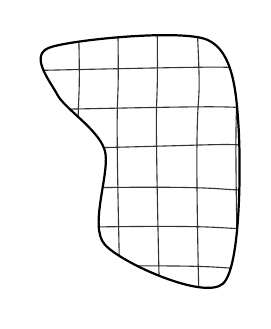
\begin{tikzpicture}
    \draw [thick] plot [smooth cycle] coordinates {(1.3, -1.2) (1.3, 0) (0.7, 0.7) (0.6, 1.3) (2.6, 1.4) (3, 0.3) (2.8, -1.7)};
    \clip plot [smooth cycle] coordinates {(1.3, -1.2) (1.3, 0) (0.7, 0.7) (0.6, 1.3) (2.6, 1.4) (3, 0.3) (2.8, -1.7)};
    \draw [step=0.5, opacity=0.8, decorate, decoration=penciline] (0, -2) grid (4, 1.7);
  \end{tikzpicture}
\end{center}
We then average out $X$ in each of these compartments to obtain $Y$. This is what we are going to call the conditional expectation of $X$ given $\mathcal{G}$, written $\E(X \mid \mathcal{G})$.

Ultimately, the characterizing property of $Y$ is the following lemma:
\begin{lemma}
  The conditional expectation $Y = \E(X \mid \mathcal{G})$ satisfies the following properties:
  \begin{itemize}
    \item $Y$ is $\mathcal{G}$-measurable
    \item We have $Y \in L^1$, and
      \[
        \E Y \mathbf{1}_A = \E X \mathbf{1}_A
      \]
      for all $A \in \mathcal{G}$.
  \end{itemize}
\end{lemma}

\begin{proof}
  It is clear that $Y$ is $\mathcal{G}$-measurable. To show it is $L^1$, we compute
  \begin{align*}
    \E[|Y|] &= \E \left|\sum_{n = 1}^\infty \E(X \mid G_n) \mathbf{1}_{G_n}\right|\\
    &\leq \E \sum_{n =1 }^\infty \E(|X| \mid G_n) \mathbf{1}_{G_n} \\
    &= \sum \E \left( \E(|X| \mid G_n) \mathbf{1}_{G_n}\right)\\
    &= \sum \E |X| \mathbf{1}_{G_n}\\
    &= \E \sum |X| \mathbf{1}_{G_n}\\
    &= \E |X|\\
    &< \infty,
  \end{align*}
  where we used monotone convergence twice to swap the expectation and the sum.

  The final part is also clear, since we can explicitly enumerate the elements in $\mathcal{G}$ and see that they all satisfy the last property.
\end{proof}

It turns out for any $\sigma$-subalgebra $\mathcal{G} \subseteq \mathcal{F}$, we can construct the conditional expectation $\E(X \mid \mathcal{G})$, which is uniquely characterized by the above two properties.

\begin{thm}[Existence and uniqueness of conditional expectation]
  Let $X \in L^1$, and $\mathcal{G} \subseteq \mathcal{F}$. Then there exists a random variable $Y$ such that
  \begin{itemize}
    \item $Y$ is $\mathcal{G}$-measurable
    \item $Y \in L^1$, and $\E X \mathbf{1}_A = \E Y \mathbf{1}_A$ for all $A \in \mathcal{G}$.
  \end{itemize}
  Moreover, if $Y'$ is another random variable satisfying these conditions, then $Y' = Y$ almost surely.

  We call $Y$ a (version of) the conditional expectation given $\mathcal{G}$.
\end{thm}

We will write the condition expectation as $\E(X \mid \mathcal{G})$, and if $X = \mathbf{1}_A$, we will write $\E(A \mid \mathcal{G}) = \E(\mathbf{1}_A \mid \mathcal{G})$.

Recall also that if $Z$ is a random variable, then $\sigma(Z) = \{Z^{-1}(B): B \in \mathcal{B}\}$. In this case, we will write $\E[X \mid Z) = \E(X \mid \sigma(Z))$.

By, say, bounded convergence, it follows from the second condition that $\E XZ = \E YZ$ for all bounded $\mathcal{G}$-measurable functions $Z$.
\begin{proof}
  We first consider the case where $X \in L^2(\Omega, \mathcal{F}, \mu)$. Then we know from functional analysis that for any $\mathcal{G} \subseteq \mathcal{F}$, the space $L^2(\mathcal{G})$ is a Hilbert space with inner product
  \[
    \langle X, Y \rangle = \mu (X Y).
  \]
  In particular, $L^2(\mathcal{G})$ is a closed subspace of $L^2(\mathcal{F})$. We can then define $Y$ to be the orthogonal projection of $X$ onto $L^2(\mathcal{G})$. It is immediate that $Y$ is $\mathcal{G}$-measurable. For the second part, we use that $X - Y$ is orthogonal to $L^2(\mathcal{G})$, since that's what orthogonal projection is supposed to be. So $\E(X - Y)Z = 0$ for all $Z \in L^2(\mathcal{G})$. In particular, since the measure space is finite, the indicator function of any measurable subset is $L^2$. So we are done.

  We next focus on the case where $X \in m\mathcal{E}^+$. We define
  \[
    X_n = X \wedge n
  \]
  We want to use monotone convergence to obtain our result. To do so, we need the following result:

  \begin{claim}
    If $(X, Y)$ and $(X', Y')$ satisfy the conditions of the theorem, and $X' \geq X$ a.s., then $Y' \geq Y$ a.s.
  \end{claim}

  \begin{proof}
    Define the event $A = \{Y' \leq Y\} \in \mathcal{G}$. Consider the event $Z = (Y - Y')\mathbf{1}_A$. Then $Z \geq 0$. We then have
    \[
      \E Y' \mathbf{1}_A = \E X' \mathbf{1}_A \geq \E X \mathbf{1}_A = \E Y \mathbf{1}_A.
    \]
    So it follows that we also have $\E(Y - Y')\mathbf{1}_A \leq 0$. So in fact $\E Z = 0$. So $Y' \geq Y$ a.s.
  \end{proof}
  We can now define $Y_n = \E(X_n \mid \mathcal{G})$, picking them so that $\{Y_n\}$ is increasing. We then take $Y_\infty = \lim Y_n$. Then $Y_\infty$ is certainly $\mathcal{G}$-measurable, and by monotone convergence, if $A \in \mathcal{G}$, then
  \[
    \E X \mathbf{1}_A = \lim \E X_n \mathbf{1}_A = \lim \E Y_n \mathbf{1}_A = \E Y_\infty \mathbf{1}_A.
  \]
  Now if $\E X < \infty$, then $\E Y_\infty = \E X < \infty$. So we know $Y_\infty$ is finite a.s., and we can define $Y = Y_\infty \mathbf{1}_{Y_\infty < \infty}$.

  Finally, we work with arbitrary $X \in L^1$. We can write $X = X^+ - X^-$, and then define $Y^\pm = \E (X^\pm \mid \mathcal{G})$, and take $Y = Y^+ - Y^-$.

  Uniqueness is then clear.
\end{proof}

\begin{lemma}
  If $Y$ is $\sigma(Z)$-measurable, then there exists $h: \R \to \R$ Borel-measurable such that $Y = h(Z)$. In particular,
  \[
    \E(X \mid Z) = h(Z) \text{ a.s.}
  \]
  for some $h: \R \to \R$.
\end{lemma}
We can then define $\E(X \mid Z = z) = h(z)$. The point of doing this is that we want to allow for the case where in fact we have $\P(Z = z) = 0$, in which case our original definition does not make sense.

\begin{ex}
  Consider $X \in L^1$, and $Z: \Omega \to \N$ discrete. Compute $\E(X \mid Z)$ and compare our different definitions of conditional expectation.
\end{ex}

\begin{eg}
  Let $(U, V) \in \R^2$ with density $f_{U, V}(u, v)$, so that for any $B_1, B_2 \in \mathcal{B}$, we have
  \[
    \P(U \in B_1, V \in B_2) = \int_{B_1} \int_{b_2} f_{U, V}(u, v) \;\d u \;\d v.
  \]
  We want to compute $\E(h(V) \mid U)$, where $h: \R \to \R$ is Borel measurable. We can define
  \[
    f_U(u) = \int_\R f_{U, V} (u, v) \;\d v,
  \]
  and we define the conditional density of $V$ given $U$ by
  \[
    F_{ \mid U} (v \mid u) = \frac{f_{U, V}(u, v)}{f_U(u)}.
  \]
  We define
  \[
    g(u) = \int h(u) f_{V \mid U} (v \mid u)\;\d v.
  \]
  We claim that $\E(h(V) \mid U)$ is just $g(U)$.

  To check this, we show that it satisfies the two desired conditions. It is clear that it is $\sigma(U)$-measurable. To check the second condition, fix an $A \in \sigma(U)$. Then $A = \{(u, v): u \in B\}$ for some $B$. Then
  \begin{align*}
    \E(h(V) \mathbf{1}_A) &= \iint h(v) \mathbf{1}_{u \in B} f_{U, V} (u, v)\;\d u\;\d v\\
    &= \iint h(v) \mathbf{1}_{u \in B} f_{V \mid U}(v \mid u) f_V(u)\;\d u\;\d v\\
    &= \int g(U) \mathbf{1}_{u \in B} f_U(u) \;\d u\\
    &= \E(g(U) \mathbf{1}_A),
  \end{align*}
  as desired.
\end{eg}
The point of this example is that to compute conditional expectations, we use our intuition to guess what the conditional expectation should be, and then check that it satisfies the two uniquely characterizing properties.

\begin{eg}
  Suppose $(X, W)$ are Gaussian. Then for all linear functions $\varphi: \R^2 \to \R$, the quantity $\varphi(X, W)$ is Gaussian.

  One nice property of Gaussians is that lack of correlation implies independence. We want to compute $\E(X \mid W)$. Note that if $Y$ is such that $\E X = \E Y$, $X - Y$ is independent of $W$, and $Y$ is $W$-measurable, then $Y = \E(X \mid W)$, since
  $\E(X - Y) \mathbf{1}_A = 0$ for all $\sigma(W)$-measurable $A$.

  The guess is that we want $Y$ to be a Gaussian variable. We put $Y = aW + b$. Then $\E X = \E Y$ implies we must have
  \[
    a \E W + b = \E X.\tag{$*$}
  \]
  The independence part requires $\cov(X - Y, W) = 0$. Since covariance is linear, we have
  \[
    0 = \cov(X - Y, W) = \cov(X, W) - \cov(aW + b, W) = \cov(X, W) - a \cov(W, W).
  \]
  Recalling that $\cov(W, W) = \var(W)$, we need
  \[
    a = \frac{\cov(X, W)}{\var(W)}.
  \]
  This then allows us to use $(*)$ to compute $b$ as well. This is how we compute the conditional expectation of Gaussians.
\end{eg}

We note some immediate properties of conditional expectation. As usual, all (in)equality and convergence statements are to be taken with the quantifier ``almost surely''.
\begin{prop}\leavevmode
  \begin{enumerate}
    \item $\E(X \mid \mathcal{G}) = X$ iff $X$ is $\mathcal{G}$-measurable.
    \item $\E(\E(X \mid \mathcal{G})) = \E X$
    \item If $X \geq 0$ a.s., then $\E(X \mid \mathcal{G}) \geq 0$
    \item If $X$ and $\mathcal{G}$ are independent, then $\E(X \mid \mathcal{G}) = \E[X]$
    \item If $\alpha, \beta \in \R$ and $X_1, X_2 \in L^1$, then
      \[
        \E(\alpha X_1 + \beta X_2 \mid \mathcal{G}) = \alpha \E(X_1 \mid\mathcal{G}) + \beta \E(X_2 \mid \mathcal{G}).
      \]
    \item Suppose $X_n \nearrow X$. Then
      \[
        \E(X_n\mid \mathcal{G}) \nearrow \E(X \mid \mathcal{G}).
      \]
    \item \term{Fatou's lemma}: If $X_n$ are non-negative measurable, then
      \[
        \E\left(\liminf_{n \to \infty} X_n \mid \mathcal{G}\right) \leq \liminf_{n \to \infty} \E(X_n \mid \mathcal{G}).
      \]
    \item \emph{Dominated convergence theorem}\index{dominated convergence theorem}: If $X_n \to X$ and $Y \in L^1$ such that $Y \geq |X_n|$ for all $n$, then
      \[
        \E(X_n \mid \mathcal{G}) \to \E(X \mid \mathcal{G}).
      \]
    \item \term{Jensen's inequality}: If $c: \R \to \R$ is convex, then
      \[
        \E(c(X) \mid \mathcal{G}) \geq c(\E(X) \mid \mathcal{G}).
      \]
    \item \emph{Tower property}\index{tower property}: If $\mathcal{H} \subseteq \mathcal{G}$, then
      \[
        \E(\E(X \mid \mathcal{G}) \mid \mathcal{H}) = \E(X \mid \mathcal{H}).
      \]
    \item For $p \geq 1$,
      \[
        \|\E(X \mid \mathcal{G})\|_p \leq \|X\|_p.
      \]
    \item If $Z$ is bounded and $\mathcal{G}$-measurable, then
      \[
        \E(ZX \mid \mathcal{G}) = Z \E(X \mid \mathcal{G}).
      \]
    \item Let $X \in L^1$ and $\mathcal{G}, \mathcal{H} \subseteq \mathcal{F}$. Assume that $\sigma(X, \mathcal{G})$ is independent of $\mathcal{H}$. Then
      \[
        \E (X \mid \mathcal{G}) = \E(X \mid \sigma(\mathcal{G}, \mathcal{H})).
      \]
  \end{enumerate}
\end{prop}

\begin{proof}\leavevmode
  \begin{enumerate} % actually check these
    \item Clear.
    \item Take $A = \omega$.
    \item Shown in the proof.
    \item Clear by property of expected value of independent variables.
    \item Clear, since the RHS satisfies the unique characterizing property of the LHS.
    \item Clear from construction.
    \item Same as the unconditional proof, using the previous property.
    \item Same as the unconditional proof, using the previous property.
    \item Same as the unconditional proof.
    \item The LHS satisfies the characterizing property of the RHS
    \item Using the convexity of $|x|^p$, Jensen's inequality tells us
      \begin{align*}
        \|E(X \mid \mathcal{G})\|_p^p &= \E |\E(X \mid \mathcal{G})|^p\\
        &\leq \E (\E (|X|^p \mid \mathcal{G}))\\
        &= \E |X|^p\\
        &= \|X\|_p^p
      \end{align*}
    \item If $Z = \mathbf{1}_B$, and let $b \in \mathcal{G}$. Then
      \[
        \E(Z \E(X \mid \mathcal{G}) \mathbf{1}_A) = \E (\E (X \mid \mathcal{G}) \cdot \mathbf{1}_{A \cap B}) = \E(X \mathbf{1}_{A \cap B}) = \E(Z X \mathbf{1}_A).
      \]
      So the lemma holds. Linearity then implies the result for $Z$ simple, then apply our favorite convergence theorems.
    \item Take $B \in \mathcal{H}$ and $A \in \mathcal{G}$. Then
      \begin{align*}
        \E(\E(X \mid \sigma(\mathcal{G}, \mathcal{H}))\cdot \mathbf{1}_{A \cap B}) &= \E(X \cdot \mathbf{1}_{A \cap B})\\
        &= \E(X \mathbf{1}_A) \P(B)\\
        &= \E(\E(X \mid \mathcal{G}) \mathbf{1}_A) \P(B)\\
        &= \E(\E(X \mid \mathcal{G}) \mathbf{1}_{A \cap B})
      \end{align*}
      If instead of $A \cap B$, we had any $\sigma(\mathcal{G}, \mathcal{H})$-measurable set, then we would be done. But we are fine, since the set of subsets of the form $A \cap B$ with $A \in \mathcal{G}$, $B \in \mathcal{H}$ is a generating $\pi$-system for $\sigma(\mathcal{H}, \mathcal{G})$. \qedhere
  \end{enumerate}
\end{proof}

We shall end with the following key lemma. We will later use it to show that many of our \emph{martingales} are uniformly integrable.
\begin{lemma}
  If $X \in L^1$, then the family of random variables $Y_{\mathcal{G}} = \E(X \mid \mathcal{G})$ for all $\mathcal{G} \subseteq \mathcal{F}$ is uniformly integrable.

  In other words, for all $\varepsilon > 0$, there exists $\lambda > 0$ such that
  \[
    \E(Y_{\mathcal{G}} \mathbf{1}_{|Y_{\mathcal{G}} > \lambda|}) < \varepsilon
  \]
  for all $\mathcal{G}$.
\end{lemma}

\begin{proof}
  Fix $\varepsilon > 0$. Then there exists $\delta > 0$ such that $\E |X|\mathbf{1}_A < \varepsilon$ for any $A$ with $\P(A) < \delta$.

  Take $Y = \E (X \mid \mathcal{G})$. Then by Jensen, we know
  \[
    |Y| \leq \E(|X| \mid \mathcal{G})
  \]
  In particular, we have
  \[
    \E|Y| \leq \E|X|.
  \]
  By Markov's inequality, we have
  \[
    \P(|Y| \geq \lambda) \leq \frac{\E|Y|}{\lambda} \leq \frac{\E|X|}{\lambda}.
  \]
  So take $\lambda$ such that $\frac{\E|X|}{\lambda} < \delta$. So we have
  \[
    \E(|Y| \mathbf{1}_{|Y| \geq \lambda}) \leq \E(\E(|X| \mid \mathcal{G})\mathbf{1}_{|Y| \geq \lambda}) = \E(|X| \mathbf{1}_{|Y| \geq \lambda}) < \varepsilon
  \]
  using that $\mathbf{1}_{|Y| \geq \lambda}$ is a $\mathcal{G}$-measurable function.
\end{proof}

\section{Martingales in discrete time}
To define a martingale in the appropriate generality, we need the notion of a filtration.
\begin{defi}[Filtration]\index{filtration}
  A \emph{filtration} is a sequence of $\sigma$-algebras $(\mathcal{F}_n)_{n \geq 0}$ such that $\mathcal{F} \supseteq \mathcal{F}_{n + 1} \supseteq \mathcal{F}_n$. We define $\mathcal{F}_\infty = \sigma(\mathcal{F}_0, \mathcal{F}_1, \ldots) \subseteq \mathcal{F}$.
\end{defi}

This is supposed to model the evolution of time, where $\mathcal{F}_n$ consists of the information we have at time $t = n$. We will from now on assume $(\Omega, \mathcal{F}, \P)$ is equipped with a filtration $(\mathcal{F}_n)_{n \geq 0}$.

\begin{defi}[Stochastic process in discrete time]\index{discrete stochastic process}\index{stochastic process!discrete}
  A \emph{stochastic process} (in discrete time) is a sequence of random variables $(X_n)_{n \geq 0}$.
\end{defi}

\begin{defi}[Natural filtration]\index{natural filtration}\index{filtration!natural}
  The \emph{natural filtration} of $(X_n)_{n \geq 0}$ is given by
  \[
    \mathcal{F}_n^X = \sigma(X_1, \ldots, X_n).
  \]
\end{defi}

\begin{defi}[Adapted process]\index{adapted process}\index{stochastic process!adapted}
  We say that $(X_n)_{n \geq 0}$ is \emph{adapted} (to $(\mathcal{F}_n)_{n \geq 0}$) if $X_n$ is $\mathcal{F}_n$-measurable for all $n \geq 0$.

  This is equivalent to saying that $\mathcal{F}^X_n \subseteq \mathcal{F}_n$.
\end{defi}

\begin{defi}[Integrable process]\index{integrable process}\index{stochastic process!integrable}
  A process $(X_n)_{n \geq 0}$ is \emph{integrable} if $X_n \in L^1$ for all $n \geq 0$.
\end{defi}

\begin{defi}[Martingale]\index{martingale}
  An integrable adapted process $(X_n)_{n \geq 0}$ is a \emph{martingale} if for all $n \geq m$, we have
  \[
    \E(X_n \mid \mathcal{F}_m) = X_m.
  \]
  We say it is a \term{super-martingale} if
  \[
    \E(X_n \mid \mathcal{F}_m) \leq X_m,
  \]
  and a \term{sub-martingale} if
  \[
    \E(X_n \mid \mathcal{F}_m) \geq X_m,
  \]
\end{defi}

Note that it is enough to take $m = n - 1$ for all $n \geq 0$, using the tower property.

\subsection{Stopping time and optimal stopping}

\begin{defi}[Stopping time]\index{stopping time}
  A \emph{stopping time} is a random variable $T: \Omega \to \N_{ \geq 0} \cup \{\infty\}$ such that
  \[
    \{T \leq n\} \in \mathcal{F}_n
  \]
  for all $n \geq 0$.
\end{defi}
This means to know that at time $n$, if we want to know if $T$ has come, we can determine it using the information we have at $T$.

\begin{eg}
  If $B \in \mathcal{B}(\R)$, then we can define
  \[
    T = \inf \{n : X_n \in B\}.
  \]
  Then this is a stopping time.

  On the other hand,
  \[
    T = \sup \{n: X_n \in B\}
  \]
  is not a stopping time (in general).
\end{eg}

\begin{defi}[$\mathcal{F}_T$]\index{$\mathcal{F}_T$}
  For a stopping time $T$, define
  \[
    \mathcal{F}_T = \{A \in \mathcal{F}_\infty : A \cap \{T \leq n\} \in \mathcal{F}_n\}.
  \]
\end{defi}
One sees that this is a $\sigma$-algebra.

\begin{eg}
  If $T \equiv n$ is constant, then $F\mathcal{F}_T = \mathcal{F}_n$.
\end{eg}

\begin{defi}[$X_T$]\index{$X_T$}
  For a stopping time $T$, we define the random variable $X_T$ by
  \[
    X_T (\omega) = X_{T(\omega)}(\omega)
  \]
  on $\{T < \infty\}$, and $0$ otherwise.
\end{defi}

\begin{defi}[Stopped process]\index{stopped process}
  The \emph{stopped process} is defined by
  \[
    (X_n^T)_{n \geq 0} = (X_{T(\omega) \wedge n}(\omega))_{n \geq 0}.
  \]
\end{defi}
So we stop the process once $T$ happens.

Note that $T$ is a stopping time iff $\{t = n \} \in \mathcal{F}_n$ for all $n$, since if $T$ is a stopping time, then
\[
  \{T = n\} = \{T \leq n\} \setminus \{T \leq n - 1\},
\]
and $\{T \leq n- 1\} \in \mathcal{F}_{n - 1} \subseteq \mathcal{F}_n$. Conversely,
\[
  \{T \leq n \} = \cup_{k = 1}^n \{T = k\} \in \mathcal{F}_n.
\]
This will not be true in the continuous case.

Let's now start writing down properties of these things.

\begin{prop}\leavevmode
  \begin{enumerate}
    \item If $T, S, (T_n)_{n \geq 0}$ are all stopping times, then
      \[
        T \vee S, T \wedge S, \sup_n T_n, \inf T_n, \limsup T_n, \liminf T_n
      \]
      are all stopping times.
    \item $\mathcal{F}_T$ is a $\sigma$-algebra
    \item If $S \leq T$, then $\mathcal{F}_S \subseteq \mathcal{F}_T$.
    \item $X_T \mathbf{1}_{T < \infty}$ is $\mathcal{F}_T$-measurable.
    \item If $(X_n)$ is an adapted process, then so is $(X^T_n)_{n \geq 0}$ for any stopping time $T$.
    \item If $(X_n)$ is an integrable process, then so is $(X^T_n)_{n \geq 0}$ for any stopping time $T$.
  \end{enumerate}
\end{prop}

\begin{proof}
  Exercise.
\end{proof}
We now come to the fundamental property of martingales.
\begin{thm}[Optional stopping theorem]\index{optional stopping theorem}
  Let $(X_n)_{n \geq 0}$ be a super-martingale and $S \leq T$ \emph{bounded} stopping times. Then
  \[
    \E(X_T) \leq \E(X_S).
  \]
\end{thm}

\begin{proof}
  See proof of the next theorem.
\end{proof}
What does this theorem mean? If $X$ is a martingale, then it is both a super-martingale and a sub-martingale. So we can apply this to both $X$ and $-X$, and so we have
\[
  \E(X_T) = \E(X_S) = \E(X_0),
\]
using the fact that $0$ is a stopping time. Martingales are supposed to model fair games. If we think of a stopping time as telling us when the game should end, and $X$ as are score, then this says there is no way of picking when the game ends that changes our expected value.

What if we look at the stopping time
\[
  T = \inf \{n : X_n = 1\},
\]
and take $X$ such that $\E X_0 = 0$. Then clearly we have $\E X_T = 1$. So this tells us $T$ is not a bounded stopping time.

\begin{thm}
  The following are equivalent:
  \begin{enumerate}
    \item $(X_n)_{n \geq 0}$ is a super-martingale.
    \item For any bounded stopping times $T$ and any stopping time $S$,
      \[
        \E(X_T \mid \mathcal{F}_S) \leq X_{S \wedge T}.
      \]
    \item $(X_n^T)$ is a super-martingale for any stopping time $T$.
    \item For bounded stopping times $S, T$ such that $S \leq T$, we have
      \[
        \E X_T \leq \E X_S.
      \]
  \end{enumerate}
\end{thm}
In particular, (iv) implies (i).

\begin{proof}\leavevmode
  \begin{itemize}
    \item (ii) $\Rightarrow$ (iii): Consider $(X_n^{T'})_{ \geq 0}$ for a stopping time $T'$. To check if this is a super-martingale, we need to prove that whenever $m \leq n$,
      \[
        \E(X_{n \wedge T} \mid \mathcal{F}_m) \leq X_{m \wedge T}.
      \]
      But this follows from (ii) above by taking $S = m$ and $T = T' \wedge n$.
    \item (ii) $\Rightarrow$ (iv): Clear by the tower law.
    \item (iii) $\Rightarrow$ (i): Take $T = \infty$.
    \item (i) $\Rightarrow$ (ii): Assume $T \leq n$.
      \begin{align*}
        X_T &= X_{S \wedge T} + \sum_{S \leq k < T} (X_{k + 1} - X_T)\\
        &= X_{S \wedge T} + \sum_{n = 0}^n (X_{k + 1} - X_k) \mathbf{1}_{S \leq k < T} \tag{$*$}
      \end{align*}
      Now note that $\{S \leq k < T\} = \{S \leq k\} \cap \{T \leq k\}^c \in \mathcal{F}_k$. Let $A \in \mathcal{F}_S$. Then $A \cap \{S \leq k\} \in \mathcal{F}_k$ by definition of $\mathcal{F}_S$. So $A \cap \{S \leq k < T\} \in \mathcal{F}_k$.

      Apply $\E$ to to $(*) \times \mathbf{1}_A$. Then we have
      \[
        \E (X_T \mathbf{1}_A) = \E(X_{S \wedge T} \mathbf{1}_A) + \sum_{k = 0}^n \E(X_{k + 1} - X_k) \mathbf{1}_{A \cap \{S \leq k < T\}}.
      \]
      But for all $k$, we know
      \[
        \E(X_{k + 1} - X_k) \mathbf{1}_{A \cap \{S \leq k < T\}} \leq 0,
      \]
      since $X$ is a super-martingale. So it follows that for all $A \in \mathcal{F}_S$, we have
      \[
        \E(X_T \cdot \mathbf{1}_A) \leq \E(X_{S \wedge T} \mathbf{1}_A).
      \]
      But since $X_{S \wedge T}$ is $\mathcal{F}_{S \wedge T}$ measurable, it is in particular $\mathcal{F}_S$ measurable. So it follows that for all $A \in \mathcal{F}_S$, we have
      \[
        \E(\E (X_T \mid \mathcal{F}_S) \mathbf{1}_A) \leq \E(X_{S \wedge T} \mathbf{1}_A).
      \]
      So the result follows.
    \item (iv) $\Rightarrow$ (i): Fix $m \leq n$ and $A \in \mathcal{F}_m$. Take
      \[
        T = m \mathbf{1}_A + \mathbf{1}_{A^C}.
      \]
      One then manually checks that this is a stopping time. Now note that
      \[
        X_T = X_m \mathbf{1}_{A} + X_n \mathbf{1}_{A^C}.
      \]
      So we have
      \[
        0 \geq \E(X_n) - \E(X_T) = \E(X_n) - \E(X_n \mathbf{1}_A) - \E(X_m \mathbf{1}_!).
      \]
      Then the same argument as before gives the result.\qedhere
  \end{itemize}
\end{proof}

\subsection{Almost sure convergence of martingales}

\begin{thm}[Almost sure martingale convergence theorem]\index{martingale convergence theorem!almost sure}
  Suppose $(X_n)_{n \geq 0}$ is a super-martingale that is bounded in $L^1$, i.e.\ $\sup_n \E|X_n| < \infty$. Then there exists an $\mathcal{F}_\infty$-measurable $X_\infty \in L^1$ such that
  \[
    X_n \to X_\infty\text{ a.s. as }n \to \infty.
  \]
\end{thm}

To prove this, we start with a deterministic lemma;
\begin{lemma}
  Let $(x_n)_{n \geq 0}$ be a sequence of numbers. Then $x_n$ converges in $\R$ if and only if
  \begin{enumerate}
    \item $\liminf |x_n| < \infty$
    \item For all $a, b \in \Q$ with $a < b$, the number of upcrossings of $(a, b)$ by $(x_n)$ is finite.\hfill\qedsymbol
  \end{enumerate}
\end{lemma}
An upcrossing of $(a, b)$ by $(x_n)$ is a sequence $j, j + 1, \ldots, k$ such that $x_j \leq a$ and $x_k \geq b$. Define
\[
  U_n[a, b, x] = \text{number of disjoint upcrossings contained in }\{1, \ldots, n\},
\]
and define
\[
  U[a, b, x] = \lim_{n \to \infty} U_n[a, b, x].
\]
This is what we call the number of upcrossings.

\begin{lemma}[Doob's upcrossing lemma]
  If $X_n$ is a supermartingale, then
  \[
    (b - a) \E(U_n[a, b(X_n)]) \leq \E(X_n - a)^-
  \]
\end{lemma}
If $\E|X| < \infty$, then $X$ is finite surely. We can then use stopping times to count upcrossings, and then use optional stopping.

\begin{proof}
%  If $X$ is a martingale, then $|X|$ is a positive supermartingale by Jensen's inequality.

  Assume that $X$ is a positive supermartingale. We define stopping times $S_k, T_k$ as follows:
  \begin{itemize}
    \item $T_0 = 0$
    \item $S_{k + 1} = \inf\{n: X_n \leq a, n \geq T_n\}$
    \item $T_{k + 1} = \inf\{n: X_n \geq b, n \geq S_{k + 1}\}$.
  \end{itemize}
  Given an $n$, we want to count the number of upcrossings before $n$. There are two cases we might want to distinguish:
  \begin{center}
    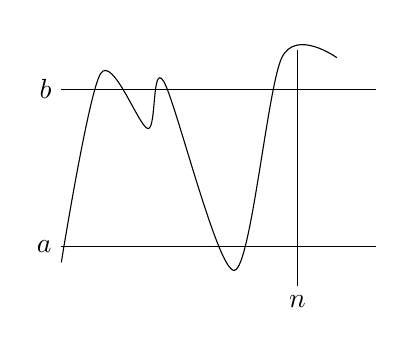
\begin{tikzpicture}
      \draw (0, 0) node [left] {$b$} -- (4, 0);
      \draw (0, -2) node [left] {$a$} -- (4, -2);
      \draw (3, -2.5) node [below] {$n$} -- (3, 0.5);

      \draw plot [smooth] coordinates {(0, -2.2) (0.5, 0.2) (1.1, -0.5) (1.3, 0.1) (2.2, -2.3) (2.8, 0.4) (3.5, 0.4)};
    \end{tikzpicture}
    \quad
    and
    \quad
    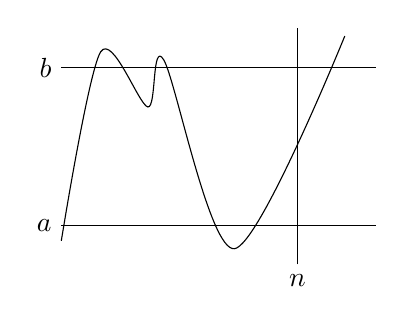
\begin{tikzpicture}
      \draw (0, 0) node [left] {$b$} -- (4, 0);
      \draw (0, -2) node [left] {$a$} -- (4, -2);
      \draw (3, -2.5) node [below] {$n$} -- (3, 0.5);

      \draw plot [smooth] coordinates {(0, -2.2) (0.5, 0.2) (1.1, -0.5) (1.3, 0.1) (2.2, -2.3) (3.6, 0.4)};
    \end{tikzpicture}
  \end{center}
  We inspect the two cases and observe that in both cases, we have
  \[
    \sum_{k = 1}^n X_{T_k \wedge n} - X_{S_k \wedge n} \geq (b - a) U_n + (X_n - X_{S_{U_n + 1} \wedge n}),
  \]
  where the second term on the right is needed for the second case.

  By super-martingale optional stopping, we have
  \[
    0 \geq (b - a) \E U_n + \E(X_n - X_{S_{U_n + 1} \wedge n}).
  \]
  Then observe that
  \[
    \E(X_n- X_{S_{U_n + 1}}) \geq - (X_n - a)^-.
  \]
\end{proof}

\begin{proof}[Proof of theorem]
  Define
  \[
    \Omega_\infty = \{\omega: \limsup (X_n(\omega))< \infty\}.
  \]
  Moreover, for all $a < b \in \R$, define
  \[
    \Omega_{a, b} = \{\omega: U[a, b, (X_n)] < \infty\}.
  \]
  By our lemma, we know that $X_n$ converges on
  \[
    \Omega_\infty \cap \left(\cap_{a < b \in \Q} \Omega_{a, b}\right).
  \]
  Moreover, by Doob's upcrossings lemma, we know
  \[
    \P\left(\Omega_\infty \cap \left(\cap_{a < b \in \Q} \Omega_{a, b}\right)\right) = 1
  \]
  since we are taking a countable intersection.
\end{proof}

This is one of the nicest theorems in this course. It says that the constraints we put on (super-)martingales are rather strong. But this is not the strongest result we will get in this course. Often, we want to have convergence of moments as well.

\begin{eg}
  Suppose $(\rho_n)_{n \geq 0}$ is a sequence of iid random variables and
  \[
    \P(\rho_n = 0) = \frac{1}{2} = \P(\rho_n = 2).
  \]
  Let
  \[
    X_n = \prod_{k = 0}^n \rho_k.
  \]
  Then this is a martingale, and $\E X_n = 1$. On the other hand, $X_n \to 0$ almost surely. So $\|X_n - X_\infty\|_1$ does not converge to $0$.
\end{eg}

To prove statements about convergence of moments, we need some inequalities.
\subsection{Doob's inequalities}
\begin{lemma}[Maximal inequality]\index{maximal inequality}
  Let $(X_n)$ be a submartingale that is non-negative, or a martingale. Define
  \[
    X^*_n = \sup_{k \leq n} |X_k|,\quad X^* = \lim_{n \to \infty} X_n^*.
  \]
  If $\lambda \geq 0$, then
  \[
    \lambda \P(X_n^* \geq \lambda) \leq \E[|X_n|\mathbf{1}_{X_n^* \geq \lambda}].
  \]
  In particular, since $X_n \geq 0$, we have
  \[
    \lambda \P(X_n^* \geq \lambda) \leq \E[|X_n|].
  \]
\end{lemma}
Markov's inequality says almost the same thing, but has $\E[|X_n^*|]$ instead of $\E[|X_n|]$. So this is a stronger inequality.

\begin{proof}
  If $X_n$ is a martingale, then $|X_n|$ is a submartingale. So it suffices to consider the case of a non-negative submartingale. We define the stopping time
  \[
    T = \inf\{n: X_n \geq \lambda\}.
  \]
  By optional stopping,
  \begin{align*}
    \E X_n &\geq \E X_{T \wedge n} \\
    &= \E X_T \mathbf{1}_{T \leq n} + \E X_n \mathbf{1}_{T > n}\\
    &\geq \lambda \P(T \leq n) + \E X_n \mathbf{1}_{T > n}\\
    &= \lambda \P(X_n^* \geq \lambda) + \E X_n \mathbf{1}_{T > n}.
  \end{align*}
\end{proof}

\begin{lemma}[$L^p$ inequality]\index{$L^p$ inequality}
  For $p > 1$, we have
  \[
    \|X_n^*\|_p \leq \frac{p}{p - 1} \|X_n\|_p
  \]
  for all $n$.
\end{lemma}

\begin{proof}
  Let $k > 0$, and consider
  \[
    \|X_n^* \wedge k \|^p_p = \E |X_n^* \wedge k|^p.
  \]
  We use the fact that
  \[
    x^p = \int_0^x p s^{p - 1}\;\d s.
  \]
  So we have
  \begin{align*}
    \|X_n^* \wedge k\|^p_p &= \E|X_n^* \wedge k|^p\\
    &= \E \int_0^{X_n^* \wedge k} p x^{p - 1}\;\d x\\
    &= \E \int_0^k p x^{p - 1} \mathbf{1}_{X_n^* \geq x}\;\d x\\
    &= \int_0^k p x^{p - 1} \P(X_n^* \geq x)\;\d x\tag{Fubini}\\
    &\leq \int_0^k px^{p - 2} \E X_n \mathbf{1}_{\{x_n^* \geq x\}} \;\d x\tag{maximal inequality}\\
    &= \E X_n \int_0^k p x^{p - 2} \mathbf{1}_{X_n^* \geq x}\;\d x \tag{Fubini}\\
    &= \frac{p}{p - 1} \E X_n (X_n^* \wedge k) ^{p - 1}\\
    &\leq \frac{p}{p - 1} \|X_n\|_p \left(\E(X_n^* \wedge k)^p\right)^{\frac{p - 1}{p}}\tag{H\:older}\\
    &= \frac{p}{p - 1} \|X_n\|_p \|X_n^* \wedge k\|_p^{p - 1}
  \end{align*}
  Now take the limit $k \to \infty$ and divide by $\|X_n^*\|_p^{p - 1}$.
\end{proof}

\begin{thm}[$L^p$ martingale convergence theorem]\index{martingale convergence theorem!$L^p$}
  Let $(X_n)_{n \geq 0}$ be a martingale, and $p > 1$. Then the following are equivalent:
  \begin{enumerate}
    \item $(X_n)_{n \geq 0}$ is bounded in $L^p$, i.e.\ $\sup_n \E |X_i|^p < \infty$.
    \item $(X_n)_{n \geq 0}$ converges as $n \to \infty$ to a random variable $X_\infty \in L^p$ almost surely and in $L^p$.
    \item There exists a random variable $Z \in L^p$ such that
      \[
        X_n = \E (Z \mid \mathcal{F}_n)
      \]
  \end{enumerate}
  Moreover, in (iii), we always have $X_\infty = \E(Z \mid \mathcal{F}_\infty)$.
\end{thm}
This gives a bijection between martingales bounded in $L^p$ and $L^p(\mathcal{F}_\infty)$, sending $(X_n)_{n \geq 0} \mapsto X_\infty$.

\begin{proof}\leavevmode
  \begin{itemize}
    \item (i) $\Rightarrow$ (ii): If $(X_n)_{n \geq 0}$ is bounded in $L^p$, then it is bounded in $L^1$. So by the martingale convergence theorem, we know $(X_n)_{n \geq 0}$ converges almost surely to $X_\infty$. By Fatou's lemma, we have $X_\infty \in L^p$.

      Now by monotone convergence, we have
      \[
        \|X^*\|_p = \lim_n \|X_n^*\|_p \leq \frac{p}{p - 1} \sup_n \|X_n\|_p < \infty.
      \]
      By the triangle inequality, we have
      \[
        |X_n - X_\infty| \leq 2 X^*\text{ a.s.}
      \]
      So by dominated convergence, we know that $X_n \to X_\infty$ in $L^p$.
    \item (ii) $\Rightarrow$ (iii): Take $Z = X_\infty$. We want to prove that
      \[
        X_m = \E(X-\infty \mid \mathcal{F}_m).
      \]
      To do so, we show that $\|X_m - \E(X_\infty \mid \mathcal{F}_m)\|_p$. For $n \geq m$, we know this is equal to
      \[
        \|E(X_n \mid \mathcal{F}_m) - \E(X_\infty \mid \mathcal{F}_m)\|_p = \|\E(X_n - X_\infty \mid \mathcal{F}_m)\|_p \leq \|X_n - X_\infty\|_p \to 0
      \]
      as $n \to \infty$, where the last step uses Jensen's. But it is also a constant. So we are done.
    \item (iii) $\Rightarrow$ (i): We need to show that if $Z \in L^p$, then $(X_n)_{n \geq 0}$ is bounded in $L^p$. % what are we actually doing?

      Note that $\bigcup_{n \geq 0} \mathcal{F}_n$ is a $\pi$-system that generates $\mathcal{F}_\infty$. So it is enough to prove that
      \[
        \E X_\infty \mathbf{1}_A = \E(\E(Z \mid \mathcal{F}_\infty) \mathbf{1}_A).
      \]
      But if $A \in \mathcal{F}_N$, then
      \begin{align*}
        \E X_\infty \mathbf{1}_A &= \lim_{n \to \infty} \E X_n \mathbf{1}_A\\
        &= \lim_{n \to \infty} \E(\E(Z \mid \mathcal{F}_n) \mathbf{1}_A)\\
        &= \lim_{n \to \infty} \E (\E(Z \mid \mathcal{F}_\infty)\mathbf{1}_A),
      \end{align*}
      where the last step relies on the fact that $\mathbf{1}_A$ is $\mathcal{F}_n$-measurable.
  \end{itemize}
\end{proof}

When $p = 1$, we cannot apply Doob's inequality. It turns out we need to impose a stronger condition.
\begin{thm}[Convergence in $L^1$]
  Let $(X_n)_{n \geq 0}$ be a martingale. Then the following are equivalent:
  \begin{enumerate}
    \item $(X_n)_{n \geq 0}$ is uniformly integrable.
    \item $(X_n)_{n \geq 0}$ converges almost surely and in $L^1$.
    \item There exists $Z \in L^1$ such that $X_n = \E(Z \mid \mathcal{F}_n)$ almost surely.
  \end{enumerate}
  Moreover, $X_\infty = \E(Z \mid F_\infty)$.
\end{thm}

The proof is very similar to the $L^p$ case.
\begin{proof}\leavevmode
  \begin{itemize}
    \item (i) $\Rightarrow$ (ii): Let $(X_n)_{n \geq 0}$ is uniformly integrable, then $(X_n)_{n \geq 0}$ is bounded in $L^1$. So the $(X_n)_{n \geq 0}$ converges to $X_\infty$ almost surely. Then by measure theory, uniform integrability implies that in fact $X_n \to L^1$.
    \item (ii) $\Rightarrow$ (iii): Same as the $L^p$ case.
    \item (iii) $\Rightarrow$ (i): For any $Z \in L^1$, the collection $\E(Z \mid \mathcal{G})$ ranging over all $\sigma$-subalgebras $\mathcal{G}$ is uniformly integrable.
  \end{itemize}
\end{proof}
Thus, note that there is a bijection between uniformly integrable martingales and $L^1(\mathcal{F}_\infty)$.

We now revisit optional stopping for uniformly integrable martingales. Recall that in the statement of optional stopping, we needed our stopping times to be bounded. It turns out if we require our martingales to be uniformly integrable, then we can drop this requirement.

\begin{thm}
  If $(X_n)_{n \geq 0}$ is a uniformly integrable martingale, and $S, T$ are arbitrary stopping times, then
  \begin{enumerate}
    \item $\E(X_T \mid \mathcal{F}_S) = X_{S \wedge T}$
    \item $\E X_T = X_0$.
  \end{enumerate}
\end{thm}
Note that we are now allowing arbitrary stopping times, so $T$ may be infinite with non-zero probability. Hence we define
\[
  X_T = \sum_{n = 0}^\infty X_n \mathbf{1}_{T = n} + X_\infty \mathbf{1}_{T = \infty}.
\]

\begin{proof}
  We'll prove that the stopped process $(X^T_n)_{n \geq 0} = (X_{T \wedge n})_{n \geq 0}$ is uniformly integrable. To see this, first note that since $(X_n)_{n \geq 0}$ is uniformly integrable, it in particular converges almost surely and in $L^1$ to $X_\infty$. Moreover, we know that$X_n = \E(X_\infty \mid \mathcal{F}_n)$. By optional stopping, we have
  \begin{align*}
    X_{T\wedge n} &= \E(X_n \mid \mathcal{F}_{T \wedge n})\\
    &= \E(\E(X_\infty \mid \mathcal{F}_n) \mid \mathcal{F}_{T \wedge n})\\
    &= \E(X_\infty \mid \mathcal{F}_{T \wedge n}).
  \end{align*}
  So we know $(X_n^T)_{n \geq 0}$ is uniformly integrable. We know $X_{n \wedge T} \to X_T$, and hence this converges in $L^1$ as well.

  We know that
  \[
    \|\E(X_{n \wedge T} - X_T \mid \mathcal{F}_S)\|_1 \leq \|X_{n \wedge T} - X_T \|_1 \to 0\text{ as }n \to \infty.
  \]
  So it follows that $\E(X_{n \wedge T} \mid \mathcal{F}_S) \to \E(X_T \mid \mathcal{F}_S)$ as $n \to \infty$.

  By optional stopping again, we know
  \[
    \E(X_{n \wedge T} \mid \mathcal{F}_S) = X_{S \wedge T \wedge n}.
  \]
  Then take the limit as $n \to \infty$.
\end{proof}

Before we go into applications, we consider the notion of a \emph{backwards martingale}.
\begin{defi}[Backwards filtration]\index{backwards filtration}\index{filtration!backwards}
  A \emph{backwards filtration} on a measurable space $(E, \mathcal{E})$ is a sequence of $\sigma$-algebras $\hat{\mathcal{F}}_n \subseteq \mathcal{E}$ such that $\hat{F}_{n + 1} \subseteq \hat{F}_n$. We define
  \[
    \hat{F}_\infty = \bigcap_{n \geq 0} \hat{F}_n.
  \]
\end{defi}

\begin{thm}
  Let $Y \in L^1$, and let $\hat{\mathcal{F}}_n$ be a backwards filtration. Then
  \[
    \E(Y \mid \hat{F}_n) \to \E(Y \mid \hat{F}_\infty)
  \]
  almost surely and in $L^1$.
\end{thm}
A process of this form is known as a \term{backwards martingale}.

\begin{proof}
  We first show that $\E(Y \mid \hat{F}_n)$ converges. We then show that what it converges to is indeed $\E(Y \mid \hat{\mathcal{F}}_\infty)$.

  We write
  \[
    X_n = \E(Y \mid \hat{\mathcal{F}}_n).
  \]
  Observe that for all $n \geq 0$, the process $(X_{n - k})_{0 \leq k \leq n}$ is a martingale by the tower property, and so is $(-X_{n - k})_{0 \leq k \leq n}$. Now notice that for all $a < b$, the number of upcrossings of $[a, b]$ by $(X_k)_{0 \leq k \leq n}$ is equal to the number of upcrossings of $[-b, -a]$ by $(-X_{n - k})_{0 \leq k \leq n}$.

  Using the same arguments as for martingales, we conclude that $X_n \to X_\infty$ almost surely and in $L^1$ for some $X_\infty$.

  To see that $X_\infty = \E(Y \mid \hat{\mathcal{F}}_\infty)$, we notice that $X_\infty$ is $\hat{F}_\infty$ measurable. So it is enough to prove that
  \[
    \E X_\infty \mathbf{1}_A = \E(\E(Y \mid \hat{\mathcal{F}}_\infty) \mathbf{1}_A)
  \]
  for all $A \in \hat{\mathcal{F}}_\infty$. Indeed, we have
  \begin{align*}
    \E X_\infty \mathbf{1}_A &= \lim_{n \to \infty} \E X_n \mathbf{1}_A\\
    &= \lim_{n\to \infty} \E(\E (Y \mid \hat{\mathcal{F}}_n) \mathbf{1}_A)\\
    &= \lim_{n \to \infty} \E(Y \mid \mathbf{1}_A)\\
    &= \E(Y \mid \mathbf{1}_A)\\
    &= \E(\E (Y \mid \hat{\mathcal{F}}_n) \mathbf{1}_A).\qedhere
  \end{align*}
\end{proof}

\subsection{Applications of martingales}
\begin{thm}[Kolmogorov 0-1 law]\index{Kolmogorov 0-1 law}
  Let $(X_n)_{n \geq 0}$ be independent random variables. Then, let
  \[
    \hat{\mathcal{F}}_n = \sigma (X_{n + 1}, X_{n + 2}, \ldots).
  \]
  $\hat{\mathcal{F}}_\infty$ is the \term{tail $\sigma$-algebra}, and th theorem is that it is trivial, i.e.\ $\P(A) \in \{0, 1\}$ for all $A \in \hat{\mathcal{F}}_\infty$.
\end{thm}

\begin{proof}
  Let $\mathcal{F}_n = \sigma(X_1, \ldots, X_n)$. Then $\mathcal{F}_n$ and $\hat{\mathcal{F}}_n$ are independent. The for all $A \in \hat{\mathcal{F}}_\infty$, we have
  \[
    \E(A \mid \mathcal{F}_n) = \P(A).
  \]
  But the LHS is a martingale. So It converges almost surely and in $L^1$ to a random variable $Y_\infty \in \mathcal{F}_\infty$. So this is just $\E(A \mid \mathcal{F}_\infty)$. But $A$ is $\mathcal{F}_\infty$-measurable, since $\hat{\mathcal{F}}_\infty \subseteq \mathcal{F}_\infty$. So this is just $\mathbf{1}_A$. So $\mathbf{1}_A = \P(A)$, and we are done.
\end{proof}

\begin{thm}[Strong law of large numbers]
  Let $(X_n)_{n \geq 1}$ be iid random variables in $L^1$, with $\E X_1 = \mu$. Define
  \[
    S_n = \sum_{i = 1}^n X_i.
  \]
  Then
  \[
    \frac{S_n}{n} \to \mu\text{ as }n \to \infty
  \]
  almost surely and in $L^1$.
\end{thm}

\begin{proof}
  We have
  \[
    S_n = \E(S_n \mid S_n) = \sum_{i = 1}^n \E(X_i \mid S_n) = n \E(X_1 \mid S_n).
  \]
  So the problem is equivalent to showing that $\E(X_1 \mid S_n) \to \mu$ as $n \to \infty$. This seems like something we can tackle with our existing technology, except that the $S_n$ do not form a filtration.

  Thus, define a backwards filtration
  \[
    \hat{\mathcal{F}}_n = \sigma(S_n, S_{n + 1}, S_{n + 2}, \ldots) = \sigma(S_n, X_{n + 1}, X_{n + 2}, \ldots) = \sigma(S_n, \tau_n),
  \]
  where $\tau_n = \sigma(X_{n + 1}, X_{n + 2}, \ldots)$. We now use the property of conditional expectation that we've never used so far, that adding independent information to a conditional expectation doesn't change the result. Since $\tau_n$ is independent of $\sigma(X_1, S_n)$, we know
  \[
    \frac{S_n}{n} = \E(X_1 \mid S_n) = \E(\hat{\mathcal{F}}_n).
  \]
  Thus, by backwards martingale convergence, we know
  \[
    \frac{S_n}{n} \to \E(X_1 \mid \hat{F}_{\infty}).
  \]
  But by the Kolmogorov 0-1 law, we know $\hat{F}_{\infty}$ is trivial. So we know that $\E(X_1 \mid \hat{F}_{\infty})$ is almost constant, which as to be $\E(\E(X_1 \mid \hat{F}_{\infty})) = \E(X_1) = \mu$.
\end{proof}

Recall that if $(E, \mathcal{E}, \mu)$ is a measure space and $f \in m\mathcal{E}^+$, then
\[
  \nu(A) = \mu(f \mathbf{1}_A)
\]
is a measure on $\mathcal{E}$. We say $f$ is a density of $\nu$ with respect to $\mu$.
We can ask an ``inverse'' question -- given two different measures on $\mathcal{E}$, when is it the case that one is given by a density with respect to the other?

A first observation is that if $\nu(A) = \mu(f \mathbf{1}_A)$, then whenever $\mu(A) = 0$, we have $\nu(A) = 0$. There is another condition which is perhaps a bit less natural. Let $\mu$ be a counting measure on $\R$, and $\nu$ the Lebesgue measure. Then our first condition is satisfied. However, if $\nu$ is given by a density $f$ with respect to $\nu$, we must have
\[
  0 = \nu(\{x\}) = \mu(f \mathbf{1}_{\{x\}}) = f(x).
\]
So $f \equiv 0$, but taking $f \equiv 0$ clearly doesn't give the Lebesgue measure.

The problem with this is that $\mu$ is not a $\sigma$-finite measure.

\begin{thm}[Radon--Nikodym]
  Let $(\Omega, \mathcal{F})$ be a measurable space, and $\Q$ and $\P$ be two probability measures on $(\Omega, \mathcal{F})$. Then the following are equivalent:
  \begin{itemize}
    \item $\Q$ is absolutely continuous with respect to $\P$, i.e.\ for any $A \in \mathcal{F}$, if $\P(A) = 0$, then $\Q(A) = 0$
    \item For any $\varepsilon > 0$, there exists $\delta > 0$ such that for all $A \in \mathcal{F}$, if $\P(A) \leq \delta$, then $\Q(A) \leq \varepsilon$.
    \item There exists a random variable $X \geq 0$ such that
      \[
        \Q(A) = \E_{\P}(X \mathbf{1}_A).
      \]
      In this case, $X$ is called the \term{Radon--Nikodym derivative} of $\Q$ with respect to $\P$, and we write $X = \frac{\d \Q}{\d \P}$.
  \end{itemize}
\end{thm}
Note that this theorem works for all finite measures by scaling, and thus for $\sigma$-finite measures by partitioning $\Omega$ into sets of finite measure.

We only treat the case where $\mathcal{F}$ is \emph{countably generated}\index{countably generated $\sigma$-algebra}\index{$\sigma$-algebra!countably generated}, i.e.\ $\mathcal{F} = \sigma(F_1, F_2, \ldots)$ for some sets $F_i$. For example, any second-countable topological space is countably generated.
\begin{proof}\leavevmode
  \begin{itemize}
    \item (ii) $\Rightarrow$ (iii): Define the filtration
      \[
        \mathcal{F}_n = \sigma(F_1, F_2, \ldots, F_n).
      \]
      Since $\mathcal{F}_n$ is finite, we can write it as
      \[
        \mathcal{F}_n = \sigma(A_{n, 1}, \ldots, A_{n, m_n}), 
      \]
      where each $A_{n, i}$ is an \term{atom}, i.e.\ if $B \subsetneq A_{n, i}$ and $b \in \mathcal{F}_n$, then $B = \emptyset$. We define
      \[
        X_n = \sum_{n = 1}^{m_n} \frac{\Q(A_{n, i})}{\P(A_{n, i})} \mathbf{1}_{A_{n, i}},
      \]
      where we skip over the terms where $\P(A_{n, i}) = 0$. We see that $(X_n)_{n \geq 0}$ are adapted. Notice that $(X_n)_{n \geq 0}$ is a martingale. Indeed, take $A \in \mathcal{F}_n$. Then (taking expectations with respect to $\P$)
      \begin{align*}
        \E X_{n + 1} \mathbf{1}_A &= \E \sum_{A_{n + 1, i} \subseteq A} \frac{\Q(A_{n + 1, i}}{\P(A_{n + 1, i})} \mathbf{1}_{n + 1, i} \\
        &= \Q(A)\\
        &= \E \sum_{A_{n, 1} \subseteq A} \frac{\Q(A_n, 1)}{\P(A_n, 1)} \mathbf{1}_{A_{n, i}}\\
        &= \E X_n \mathbf{1}_A.
      \end{align*}
      So we know that
      \[
        \E(X_{n + 1} \mid \mathcal{F}_n) = X_n.
      \]
      We shall show that $(X_n)_{n \geq 0}$ are uniformly integrable. By Markov's inequality, we have
      \[
        \P(X_n \geq \lambda) \leq \frac{\E X_n}{\lambda} = \frac{1}{\lambda}\leq \delta
      \]
      for $\lambda$ large enough. Then
      \[
        \E(X_n \mathbf{1}_{X_n \geq \lambda}) = \Q(X_n \geq \lambda) \leq \varepsilon.
      \]
      So we have shown uniform integrability, and so we know $X_n \to X$ almost surely and in $L^1$. Then for all $A \in \bigcup_{n \geq 0} \mathcal{F}_n$, we have
      \[
        \Q(A) = \lim_{n \to \infty} \E X_n \mathbf{1}_A = \E X \mathbf{1}_A.
      \]
      So $\Q(-)$ and $\E X \mathbf{1}_{(-)}$ agree on $\bigcup_{n \geq 0} \mathcal{F}_n$, which is a generating $\pi$-system for $\mathcal{F}$, so they must be the same.
    \item (i) $\Rightarrow$ (ii): Suppose not. Then there exists some $\varepsilon > 0$ and some $A_1, A_2, \ldots \in \mathcal{F}$ such that
      \[
        \Q(A_n) \geq \varepsilon,\quad \P(A_n) \leq \frac{1}{2^n}.
      \]
      Since $\sum_n \P(A_n)$ is finite, by Borel--Cantelli, we know
      \[
        \P \limsup A_n = 0.
      \]
      On the other hand, by, say, dominated convergence, we have
      \begin{align*}
        \Q\limsup A_n &= \Q \left(\bigcap_{n = 1}^\infty \bigcup_{m = n}^\infty A_m\right) \\
        &= \lim_{k \to \infty} \Q\left(\bigcap_{n = 1}^k \bigcup_{m = n}^\infty A_m \right)\\
        &\geq \lim_{k \to \infty} \Q \left(\bigcup_{m = k}^\infty A_k\right)\\
        &\geq \varepsilon.
      \end{align*}
      This is a contradiction.
  \end{itemize}
\end{proof}

\subsection{Markov chains}
Let $E$ be a countable space, and $\mu$ a measure on $E$. We write $\mu_x = \mu(\{x\})$, and then $\mu(f) = \mu \cdot f$.

\begin{defi}[Transition matrix]\index{transition matrix}
  A \emph{transition matrix} is a matrix $P = (p_{xy})_{x, y \in E}$ such that each $p_x = (p_{x, y})_{y \in E}$ is a probability measure on $E$.
\end{defi}

\begin{defi}[Markov chain]\index{Markov chain}
  An adapted process $(X_n)$ is called a \emph{Markov chain} if for any $n$ and $A \in \mathcal{F}_n$ and $\{x_n = x\} \supseteq A$, then
  \[
    \P(X_{n + 1} = y\mid A) = p_{xy}.
  \]
\end{defi}

\begin{defi}[Harmonic function]\index{harmonic function}
  A function $f: E \to \R$ is \emph{harmonic} if $Pf = f$. In other words, for any $x$, we have
  \[
    \sum_{y} p_{xy} f(y) = f(x).
  \]
\end{defi}
We then observe that

\begin{prop}
  if $F$ is harmonic and bounded, and $(X_n)_{n \geq 0}$ is Markov, then $(f(x_n))_{n \geq 0}$ is a martingale.
\end{prop}

\begin{eg}
  Let $(X_n)_{n \geq 0}$ be iid $\Z$-valued random variables in $L^1$, and $\E[X_i] = 0$. Then
  \[
    S_n = X_0 + \cdots + _n
  \]
  is a martingale and a Markov chain.

  However, if $Z$ is a $\Z$-valued random variable, consider the random variable $(ZS_n)_{n \geq 0}$ and $\mathcal{F}_n = \sigma(\mathcal{F}_n^\times, \Z)$. Then this is a martingale but not a Markov chain.
\end{eg}

\section{Continuous time stochastic processes}
\begin{defi}[Continuous time stochastic process]\index{continuous time stochastic process}\index{stochastic process}
  A \emph{continuous time stochastic process} is a family of random matrices $(X_t)_{t \geq 0}$ (or $(X_t)_{t \in [a, b]}$).
\end{defi}

In the discrete case, if $T$ is a random variable taking values in $\{0, 1, 2, \ldots\}$, then it makes sense to look at the new random variable $X_T$, since this is just
\[
  X_T = \sum_{n = 0}^\infty X_n \mathbf{1}_{T = n}.
\]
This is obviously measurable, since it is a limit of measurable functions.

However, this is not necessarily the case if we have continuous time, unless we assume some regularity conditions on our process. In some sense, we want $X_t$ to depend ``continuously'' or at least ``measurably'' on $t$.

It would be enough to require that the map
\[
  \varphi: (\omega, t) \mapsto X_t(\omega)
\]
is measurable when we put the product $\sigma$-algebra on the domain.

In this case, $X_T(\omega) = \varphi(\omega, T(\omega))$ is measurable. In this formulation, we see why we didn't have this problem with discrete time --- the $\sigma$-algebra on $\N$ is just $\P(\N)$, and so all sets are measurable. This is not true for $\mathcal{B}([0, \infty))$.

While measurability is enough, we will require something slightly stronger.

\begin{defi}[Cadlag function]\index{cadlag function}
  We say a function $X: [0, \infty] \to \R$ is \emph{cadlag} (continue \'a droite, limite \'a gauche) if for all $t$, $x_s \to x_t$ if $s \to t, s \geq t$, and for all $t$, there exists $x_{t^-}$ such that $x_s \to x_{t^-}$ if $s \to t$ and $s \leq t$.
\end{defi}

\begin{defi}[Continuous/Cadlag stochastic process]\index{continuous stochastic process}\index{stochastic process!continuous}\index{cadlag stochastic process}\index{stochastic process!cadlag}
  We say a stochastic process is \emph{continuous} (resp.\ cadlag) if for any $\omega \in \Omega$, the map $t \mapsto X_t (\omega)$ is continuous (resp.\ cadlag).
\end{defi}

\begin{notation}
  We write \term{$C([0, \infty), \R)$} for the space of all continuous functions $[0, \infty) \to \R$, and $D([0, \infty), \R)$ the space of all cadlag functions.

  We endow these spaces with a $\sigma$-algebra generated by the coordinate functions
  \begin{align*}
    C([0, \infty), \R) &\to \R
    (x_t)_{t \geq 0} &\mapsto x_s.
  \end{align*}
  and similarly for $D$.
\end{notation}

Then a continuous (or cadlag) process is a random variable taking values in $C([0, \infty), \R)$ (or $D([0, \infty), \R)$).

\begin{defi}[Finite-dimensional distribution]\index{finite-dimensional distribution}\index{distribution!finite-dimensional}
  A \emph{finite dimensional distribution} of $(X_t)_{t \geq 0}$ is a measure on $\R^n$ of the form
  \[
    \mu_{t_1, \ldots, t_n}(A) = \P((X_{t_1}, \ldots, X_{t_n}) \in A)
  \]
  for all $A \in \mathcal{B}(\R^n)$, for some $t_1 < t_2 < \ldots < t_n$.
\end{defi}

The important observation is that if we know all finite-dimensional distributions, then we know the law of $X$, since the cylinder sets form a $\pi$-system generating the $\sigma$-algebra.

\begin{thm}[Kolmogorov's criterion]\index{Kolmogorov's criterion}
  Let $(\rho_t)_{t \in I}$ be random variables, where $I \subseteq [0, 1]$ be dense. Assume that for some $p > 1$ and $\beta > \frac{1}{p}$
  \[
    \|\rho_t - \rho_s\|_p \leq |t - s|^\beta\tag{$*$}
  \]
  for all $t, s \in I$.

  Then there exists a continuous process $(X_t)_{t \in I}$ such that for all $t \in I$, 
  \[
    X_t = \rho_t \text{ almost surely},
  \]
  and moreover for any $\alpha \in [0, \beta - \frac{1}{p}]$, there exists a random variable $K_\alpha \in L^p$ such that
  \[
    |X_s - X_t| \leq K_\alpha |s - t|^\alpha
  \]
  for all $s, t \in [0, 1]$.
\end{thm}
The idea is to reduce the problem to a countable problem.

\begin{proof}
  Let $D_n = \{s \in [0, 1] : s = \frac{k}{2^n}\text{ for some }k \in \Z\}$. These are the \term{dyadic numbers} of order $n$, and define
  \[
    D = \bigcup_{n \geq 0}D_n.
  \]
  Taking limits in $L^p$, we extend $\rho_t$ to allow $t$ to take values in $D$ as well as $I$, and condition $(*)$ is still satisfied for all $s, t \in D \cup I$.

  Now define
  \[
    K_n = \sup_{t \in D_n} |S_{t + 2^{-n}} - S_t|.
  \]
  Note that there is a natural bound
  \[
    \E K_n^p \leq \sum_{t \in D_n}^n \E |\rho_{t + 2^{-n}} - \rho_T|^p \leq C^p 2^n \cdot 2^{-n \beta} = C 2^{n(1 - p\beta)}.
  \]
  Note that we assumed $p\beta > 1$. So this is exponentially decreasing in $n$. Now for all $\alpha \in [0, b - \frac{1}{p})$, define
  \[
    K_\alpha = 2 \sum_{n \geq 0} 2^{n\alpha} K_n.
  \]
  Then we have
  \begin{align*}
    \|K_\alpha\|_p &\leq 2 \sum_{n \geq 0}2^{n\alpha} \|K_n\|_p \\
    &\leq 2C \sum_{n \geq 0} 2^{n\alpha}\\
    &\leq 2C \sum_{n \geq 0} 2^{n\alpha} \cdot 2^{n\left(\frac{1}{p} - \beta\right)}\\
    &= 2C \sum_{n \geq 0} 2^{n(\alpha + \frac{1}{p} - \beta)} < \infty.
  \end{align*}
  Take $s < t$ with $s, t \in D$. Take $m > t$ such that
  \[
    2^{-(m + 1)} < t - s \leq 2^{-m}.
  \]
  Hence, there exists $u = \frac{k}{2^{m + 1}}$ such that $s < u < t$. Then
  \[
    u - s < 2^{-m},\quad t - u < 2^{-m}.
  \]
  Then we can write
  \begin{align*}
    u - s &= \sum_{i \geq m + 1} \frac{x_i}{2^i}\\
    t - u &= \sum_{i \geq m + 1} \frac{y_i}{2^i},
  \end{align*}
  where $x_i, y_i \in \{0, 1\}$. This implies we can bound
  \[
    |\rho_s - \rho_t| \leq 2 \sum_{n = m + 1}^\infty K_n.
  \]
  Thus, we have
  \begin{align*}
    \frac{|\rho_s - \rho_t|}{|s - t|} &\leq 2^{(n + 1)\alpha} 2 \sum_{n = m + 1}^\infty K_n\\
    &= 2^{n\alpha}K_n\\
    &\leq K_\alpha.
  \end{align*}
  Then define
  \[
    X_t = 
    \begin{cases}
      \lim_{q \in D} \rho_q & K_\alpha < \infty\\
      0 & \text{otherwise}.
    \end{cases}
  \]
\end{proof}

\begin{defi}[Continuous time filtration]\index{continuous time filtration}\index{filtration!continuous time}
  A \emph{continuous-time filtration} is a family of $\sigma$-algebras $(\mathcal{F}_t)_{t \geq 0}$ such that $\mathcal{F}_s \subseteq \mathcal{F}_t \subseteq \mathcal{F}$ if $s \leq t$.

  Define $\mathcal{F}_\infty = \sigma(\mathcal{F}_t: t \geq 0)$.\index{$\mathcal{F}_\infty$}
\end{defi}

\begin{defi}[Stopping time]\index{stopping time}\index{stopping time!continuous time}
  A random variable $t: \Omega \to [0, \infty]$ is a \emph{stopping time} iff
  \[
    \{T \leq t\} \in \mathcal{F}_t
  \]
  for all $t \geq 0$.
\end{defi}

\begin{prop}
  Let $(X_t)_{t \geq 0}$ be a cadlag adapted process and $S, T$ stopping times. Then
  \begin{enumerate}
    \item $S \wedge T$ is a stopping time.
    \item If $S \leq T$, then $\mathcal{F}_S \subseteq \mathcal{F}_T$.
    \item $X_T \mathbf{1}_{T < \infty}$ is $\mathcal{F}_T$-measurable.
    \item $(X_t^T)_{t \geq 0} = (X_{T \wedge t})_{t \geq 0}$ is adapted.
  \end{enumerate}
\end{prop}

We only prove (iii). The first two are the same as the discrete case, and the proof of (iv) is similar to that of (iii).

To prove this, we need a quick lemma, whose proof is a simple exercise.
\begin{lemma}
  A random variable $Z$ is $\mathcal{F}_T$-measurable iff $Z \mathbf{1}_{\{T \leq t\}}$ is $\mathcal{F}_t$-measurable for all $t \geq 0$.
\end{lemma}

\begin{proof}[Proof of proposition]
  We need to prove that $X_T \mathbf{1}_{\{T \leq t\}}$ is $\mathcal{F}_t$-measurable for all $t \geq 0$.

  We write
  \[
    X_T\mathbf{1}_{T \leq t} = X_T \mathbf{1}_{T < t} + X_t \mathbf{1}_{T = t}.
  \]
  We know the second term is measurable. So it suffices to show that $XX_T \mathbf{1}_{T < t}$ is $\mathcal{F}_t$-measurable.

  Define $T_n = 2^{-n} \lceil 2^n T\rceil$. This is a stopping time, since to know if $T_n$ happened, we only need to know if $T$ has happened yet, as $T_n \geq T$. Formally,
  \begin{align*}
    \{T_n \leq t\} &= \{\lceil 2^n T \rceil \leq 2^n t\} \\
    = \{2^n T \leq \lfloor 2^n t\rfloor\} \\
    &= \{T \leq 2^{-n} \lfloor 2^n t \rfloor\} \in \mathcal{F}_{2^{-n}\lfloor 2^n T\rfloor} \subseteq \mathcal{F}_t.
  \end{align*}
  Since $(X_t)_{t \geq 0}$ is cadlag, we know
  \[
    X_T \mathbf{1}_{\{T < t\}} = \lim_{n \to \infty} X_{T_n \wedge t} \mathbf{1}_{T < t}.
  \]
  Now $T_n \wedge t$ can take only countably (and in fact only finitely) many values, we can write
  \[
    X_{T_n \wedge t} = \sum_{q \in D_n, q < t} X_{q} \mathbf{1}_{T_n = q} + X_t \mathbf{1}_{T < t < T_n},
  \]
  and this is $\mathcal{F}_t$-measurable. So we are done.
\end{proof}

Let's focus on a particular class of stopping times --- hitting times, or first-visit times. This is a bit subtle.

\begin{defi}[Hitting time]\index{hitting time}
  Let $A \in \mathcal{B}(\R)$. Then the \emph{hitting time} of $A$ is
  \[
    T_A = \inf_{t \geq 0} \{X_t \leq A\}.
  \]
\end{defi}

This is not always a stopping time. For example, consider the process $X_t$ such that with probability $\frac{1}{2}$, it is given by $X_t = t$, and with probability $\frac{1}{2}$, it is given by
\[
  X_t = 
  \begin{cases}
    t & t \leq 1\\
    2 - t & t > 1
  \end{cases}.
\]
\begin{center}
  \begin{tikzpicture}
    \draw (0, 0) -- (3, 0);
    \draw (0, -1) -- (0, 3);
    \draw (0, 0) -- (1, 1);
    \draw [dashed] (1, 1) -- (3, 3);
    \draw [dashed] (1, 1) -- (3, -1);

    \draw (1, -0.02) node [below] {$1$} -- (1, 0.02);
    \draw (-0.02, 1) node [left] {$1$} -- (0.02, 1);
    
    \node [circ] at (1, 1){};
  \end{tikzpicture}
\end{center}
Then $T_A = 1$ in the first case, and $T_A = \infty$ in the second case. But $\{T_a \leq 1\} \not \in \mathcal{F}_1$, as at time $1$, we don't know if we are going up or down.

The problem is that $A$ is not closed.

\begin{prop}
  Let $A \subseteq \R$ be a closed set and $(X_t)_{t \geq 0}$ be continuous. Then $T_A$ is a stopping time.
\end{prop}

\begin{proof}
  Observe that
  \[
    \{T_A \leq t\} = \inf_{q \in \Q, q < t} d(X_q, A) = 0\}.
  \]
  Note that $d(X_q, A)$ is a continuous function in $q$. So we are done.
\end{proof}

Motivated by our previous non-example of a hitting time, we define
\begin{defi}[Right-continuous filtration]\index{filtration!right continuous}\index{right continuous filtration}
  Given a continuous filtration $(\mathcal{F}_t)_{t \geq 0}$, we define
  \[
    \mathcal{F}_{t+} = \bigcap_{s > t} \mathcal{F}_s \supseteq \mathcal{F}_t.
  \]
  We say $(\mathcal{F}_t)_{t \geq 0}$ is \emph{right continuous} if $\mathcal{F}_t = \mathcal{F}_{t+}$.
\end{defi}

We let $\mathcal{N} = \{A \in \mathcal{F}_\infty : \P(A) \in \{0, 1\}\}$. This is a $\sigma$-algebra.
\begin{defi}[Usual conditions]\index{usual conditions}
  We say that $(\mathcal{F}_t)_{t \geq 0}$ satisfies the \emph{usual conditions} if it is right continuous and $\mathcal{N} \subseteq \mathcal{F}_0$.
\end{defi}
The second condition tells us we are allowed to modify our events by things of mesaure zero.

\begin{prop}
  Let $(X_t)_{t \geq 0}$ be an adapted process (to $(\mathcal{F}_{t})_{t \geq 0}$) that is cadlag, and let $A$ be an open set. Then $T_A$ is a stopping time with respect to $\mathcal{F}_{t+}$.
\end{prop}

\begin{proof}
  Since $(X_t)_{t \geq 0}$ is cadlag and $A$ is open. Then
  \[
    \{T_A < t\} = \bigcup_{q < t, q \in \Q} \{X_q \in A\}.
  \]
  Then
  \[
    \{T_A \leq t\} = \bigcap_{n \geq 0} \left\{T_A < t + \frac{1}{n}\right\} \in \mathcal{F}_{t+}.
  \]
\end{proof}

\subsection{Continuous time martingales}
We can now talk about continuous time martingales.

\begin{defi}[Coninuous time martingale]\index{martingale!continuous time}\index{continuous time martingale}\index{sub-martingale!continuous time}\index{continuous time sub-martingale}\index{super-martingale!continuous time}\index{continuous time super-martingale}
  An adapted process $(X_t)_{t \geq 0}$ is called a \emph{martingale} iff
  \[
    \E (X_t \mid \mathcal{F})S = X_s
  \]
  for all $t \geq s$, and similarly for super-martingales and sub-martingales.
\end{defi}

Note that if $t_1 \leq t_2 \leq \cdots$, then
\[
  \tilde{X}_n = X_{t_n}
\]
is a discrete time martingale. Similarly, if $t_1 \geq t_2 \geq \cdots$, and
\[
  \hat{X}_n = X_{t_n}
\]
defines a discrete time backwards martingale.

We can now prove theorems we already know in the discrete case.

\begin{thm}[Optional stopping theorem]\index{optional stopping theorem}
  Let $(X_t)_{t \geq 0}$ be an adapted cadlag process in $L^1$. Then the following are equivalent:
  \begin{enumerate}
    \item For any bounded stopping time $T$ and any stopping time $S$, we have $X_T \in L^1$ and
      \[
        \E(X_T \mid \mathcal{F}_S) = X_{T \wedge S}.
      \]
    \item For any stopping time $T$, $(X_t^T)_{t \geq 0} = (X_{T \wedge t})_{t \geq 0}$ is a martingale.
    \item For any bounded stopping time $T$, $X_T \in L^1$ and $\E X_T = \E X_0$.
  \end{enumerate}
\end{thm}

\begin{proof}
  We show that (i) $\Rightarrow$ (ii), and the rest follows from the discrete case similarly.

  Assume $T \leq t$. Let
  \[
    T_n = 2^{-n} \lceil 2^n T\rceil,\quad S_n = 2^{-n} \lceil 2^n S\rceil.
  \]
  We have $T_n \searrow T$ as $n \to \infty$, and so $X_{T_n} \to X_T$ as $n \to \infty$.

  By discrete time optional stopping (since $(X_t)_{t \in D_n}$ is a discrete time martingale), and since $T_n \leq t + 1$, discrete time optional stopping tells us
  \[
    \E (X_{t + 1} \mid \mathcal{F}_{T_n}) = X_{T_n}.
  \]
  In particular, $X_{T_n}$ is uniformly integrable. So it converges in $L^1$. This implies $X_T \in L^1$.

  Arguing the same way for $S_n \wedge T_n$, we get
  \[
    X_{T_n \wedge S_n} \to X_{T \wedge S_n}.
  \]
  Now if $A \in \mathcal{F}_S$, we need to show that
  \[
    \E X_T \mathbf{1}_A = \E X_{S \wedge T} \mathbf{1}_A.
  \]
  But we know $\mathcal{F}_S \subseteq \mathcal{F}_{S_n}$ for all $n$.

  By $L^1$ convergence, and since $A \in \mathcal{F}_{S_n}$, this is equivalent to showing that
  \[
    \E X_T \mathbf{1}_A = \lim_{n \to \infty} \E X_{T_n} \mathbf{1}_A = \lim_{n \to \infty} \E X_{S_n \wedge T_n} \mathbf{1}_A,
  \]
  and this follows from discrete time optional stopping.
\end{proof}

\begin{thm}
  Let $(X_t)_{t \geq 0}$ be a supermartingale bounded in $L^1$. Then it converges almost surely as $t \to \infty$ to a random variable $X_\infty \in L^1$.
\end{thm}

\begin{proof}
  Let
  \[
    X^* = \sup_{t \geq 0} |X_t|,\quad X_{(n)}^* = \sup_{t \in D_n} |X_t|.
  \]
  Since $X_t$ is cadlag, and since $D_n$ are are monotone (in $n$), we can write
  \[
    X^* = \lim_{n \to \infty} X_n^*.
  \]
  Since $(X_t^{(n), *}) = (X_t)_{t \in D_n}$ is a super-martingale bounded in $L^1$, we know $X^*_{(n)}$ is bounded almost surely. So $X^*$ is finite almost surely.

  Define $U_s[a, b, (x_t)_{t \geq 0}]$ be the number of upcrossings of $[a, b]$ by $(x_t)_{t \geq 0}$ up to time $s$, and
  \[
    U_\infty[a, b, (x_t)_{t \geq 0}] = \lim_{s \to \infty} U_s.
  \]
  Then for all $s \geq 0$, we have
  \[
    U_s[a, b, (x_t)_{t \geq 0}] = \lim_{n \to \infty} U_s[a, b, (x_t^{(n)})_{t \in D_n}].
  \]
  By monotone convergence and Doob's upcrossing lemma, we have
  \[
    \E U_s[a, b, (X_t)_{t \geq 0}] = \lim_{n \to \infty} \E U_s[a, b, (X_t)_{t \in D_n}] \leq \frac{\E(X_s - a]^-}{b - 1} \leq \frac{\E |X_s| + a}{b - a}. % second X_t should be something else
  \]
  We are then done by taking the supremum over $s$.

  Then finish the argument as in the discrete case.
\end{proof}
\printindex
\end{document}
